% Options for packages loaded elsewhere
\PassOptionsToPackage{unicode}{hyperref}
\PassOptionsToPackage{hyphens}{url}
%
\documentclass[
  10pt,
  ignorenonframetext,
]{beamer}
\usepackage{pgfpages}
\setbeamertemplate{caption}[numbered]
\setbeamertemplate{caption label separator}{: }
\setbeamercolor{caption name}{fg=normal text.fg}
\beamertemplatenavigationsymbolsempty
% Prevent slide breaks in the middle of a paragraph
\widowpenalties 1 10000
\raggedbottom
\setbeamertemplate{part page}{
  \centering
  \begin{beamercolorbox}[sep=16pt,center]{part title}
    \usebeamerfont{part title}\insertpart\par
  \end{beamercolorbox}
}
\setbeamertemplate{section page}{
  \centering
  \begin{beamercolorbox}[sep=12pt,center]{part title}
    \usebeamerfont{section title}\insertsection\par
  \end{beamercolorbox}
}
\setbeamertemplate{subsection page}{
  \centering
  \begin{beamercolorbox}[sep=8pt,center]{part title}
    \usebeamerfont{subsection title}\insertsubsection\par
  \end{beamercolorbox}
}
\AtBeginPart{
  \frame{\partpage}
}
\AtBeginSection{
  \ifbibliography
  \else
    \frame{\sectionpage}
  \fi
}
\AtBeginSubsection{
  \frame{\subsectionpage}
}
\usepackage{amsmath,amssymb}
\usepackage{lmodern}
\usepackage{iftex}
\ifPDFTeX
  \usepackage[T1]{fontenc}
  \usepackage[utf8]{inputenc}
  \usepackage{textcomp} % provide euro and other symbols
\else % if luatex or xetex
  \usepackage{unicode-math}
  \defaultfontfeatures{Scale=MatchLowercase}
  \defaultfontfeatures[\rmfamily]{Ligatures=TeX,Scale=1}
\fi
\usetheme[]{AnnArbor}
\usecolortheme{dolphin}
\usefonttheme{structurebold}
% Use upquote if available, for straight quotes in verbatim environments
\IfFileExists{upquote.sty}{\usepackage{upquote}}{}
\IfFileExists{microtype.sty}{% use microtype if available
  \usepackage[]{microtype}
  \UseMicrotypeSet[protrusion]{basicmath} % disable protrusion for tt fonts
}{}
\makeatletter
\@ifundefined{KOMAClassName}{% if non-KOMA class
  \IfFileExists{parskip.sty}{%
    \usepackage{parskip}
  }{% else
    \setlength{\parindent}{0pt}
    \setlength{\parskip}{6pt plus 2pt minus 1pt}}
}{% if KOMA class
  \KOMAoptions{parskip=half}}
\makeatother
\usepackage{xcolor}
\newif\ifbibliography
\usepackage{longtable,booktabs,array}
\usepackage{calc} % for calculating minipage widths
\usepackage{caption}
% Make caption package work with longtable
\makeatletter
\def\fnum@table{\tablename~\thetable}
\makeatother
\usepackage{graphicx}
\makeatletter
\def\maxwidth{\ifdim\Gin@nat@width>\linewidth\linewidth\else\Gin@nat@width\fi}
\def\maxheight{\ifdim\Gin@nat@height>\textheight\textheight\else\Gin@nat@height\fi}
\makeatother
% Scale images if necessary, so that they will not overflow the page
% margins by default, and it is still possible to overwrite the defaults
% using explicit options in \includegraphics[width, height, ...]{}
\setkeys{Gin}{width=\maxwidth,height=\maxheight,keepaspectratio}
% Set default figure placement to htbp
\makeatletter
\def\fps@figure{htbp}
\makeatother
\setlength{\emergencystretch}{3em} % prevent overfull lines
\providecommand{\tightlist}{%
  \setlength{\itemsep}{0pt}\setlength{\parskip}{0pt}}
\setcounter{secnumdepth}{-\maxdimen} % remove section numbering
\def\begincols{\begin{columns}}
\def\begincol{\begin{column}}
\def\endcol{\end{column}}
\def\endcols{\end{columns}}
\usepackage{multicol}
\newcommand{\btwocol}{\begin{multicols}{2}}
\newcommand{\etwocol}{\end{multicols}}
\ifLuaTeX
  \usepackage{selnolig}  % disable illegal ligatures
\fi
\IfFileExists{bookmark.sty}{\usepackage{bookmark}}{\usepackage{hyperref}}
\IfFileExists{xurl.sty}{\usepackage{xurl}}{} % add URL line breaks if available
\urlstyle{same} % disable monospaced font for URLs
\hypersetup{
  pdftitle={Distribuciones Muestales},
  pdfauthor={Sergio Nava},
  hidelinks,
  pdfcreator={LaTeX via pandoc}}

\title{Distribuciones Muestales}
\author{Sergio Nava}
\date{octubre de 2022}

\begin{document}
\frame{\titlepage}

\begin{frame}[allowframebreaks]
  \tableofcontents[hideallsubsections]
\end{frame}
\hypertarget{distribuciones-muestrales}{%
\section{Distribuciones Muestrales}\label{distribuciones-muestrales}}

\begin{frame}{Muestreo}
\protect\hypertarget{muestreo}{}
\begin{itemize}
\tightlist
\item
  El muestreo es una herramienta de la investigación científica.
\item
  Su función básica es determinar que parte de una realidad en estudio
  (población o universo) debe examinarse con la finalidad de hacer
  inferencias sobre dicha población.
\end{itemize}
\end{frame}

\begin{frame}{Revisión de conceptos}
\protect\hypertarget{revisiuxf3n-de-conceptos}{}
\begin{itemize}
\item
  La información de los estudios de muestreo es parte de nuestra vida
  diaria, casi en su totalidad. Tal información determina el rumbo que
  deberán tomar algunas políticas gubernamentales como, por ejemplo, la
  promoción de programas sociales o el control de la economía
\item
  Las encuestas de opinión son la base de muchas de las noticias
  proporcionadas en los medios. Los estudios de rating televisivo
  determinan cuales son los programas que permanecerán al aire en el
  futuro.
\item
  No se diga los estudios de preferencias electorales, para definir
  estrategias por parte de los partidos políticos.
\item
  Las investigaciones de mercado indicaran cuales productos y con que
  características son los preferidos de los consumidores
\item
  Por otro lado, están los estudios de muestreo en las ciencias
  biológicas, geológicas, del medio ambiente, marítimas entre otras.
\item
  Muestreo de Aceptación (Industrial)
\end{itemize}
\end{frame}

\begin{frame}{}
\protect\hypertarget{section}{}
\begin{itemize}
\item
  Aún cuando la terminología de las ciencias sociales difiere de las
  ciencias exactas, los científicos sociales conducen estudios de
  muestreo y los científicos de las áreas físicas realizan en su mayoria
  experimentos, ambos tienen el propósito de captar información en torno
  a los fenómenos naturales.
\item
  Sin embargo, esas diferencias existen en el campo de la ciencia,
  debido a la naturaleza de las poblaciones y a la manera en que una
  muestra puede ser extraída. Por ejemplo, poblaciones de votantes, de
  cuentas financieras, o de animales de una especie particular pueden
  contener un número relativamente pequeño de elementos (finito).
\item
  En contraste, la población conceptual de respuestas generadas por la
  medición de la producción de un proceso químico, es muy grande
  (infinito). Las limitaciones del procedimiento de muestreo también
  varían de un área de la ciencia a otra.
\item
  El muestreo en las ciencias biológicas y físicas, puede frecuentemente
  ser realizado bajo condiciones experimentales controladas. Tal control
  es frecuentemente imposible en las ciencias sociales, negocios, y
  administración de recursos naturales (observación).
\end{itemize}
\end{frame}

\begin{frame}{Un ejemplo: Población y muestra}
\protect\hypertarget{un-ejemplo-poblaciuxf3n-y-muestra}{}
\begin{block}{¿Cómo realizar un inventario?}
\protect\hypertarget{cuxf3mo-realizar-un-inventario}{}
\begin{enumerate}
\tightlist
\item
  Censo: es un conteo exhaustivo de los individuos o elementos de la
  población bajo estudio.
\end{enumerate}

Desventajas:

\begin{itemize}
\item
  Costos elevados.
\item
  Estático
\item
  Requiere mucho tiempo
\end{itemize}

\begin{enumerate}
\setcounter{enumi}{1}
\tightlist
\item
  Muestreo: una parte representativa del recurso.
\end{enumerate}

Ventajas:

\begin{itemize}
\item
  Reduce costos.
\item
  Puede ser dinámico
\item
  Reduce tiempos.
\end{itemize}
\end{block}
\end{frame}

\begin{frame}{Conceptos de Población y Muestra}
\protect\hypertarget{conceptos-de-poblaciuxf3n-y-muestra}{}
\begin{itemize}
\item
  Se ha manejado que la estadística moderna es la teoría de la
  información, cuyo objetivo es la \emph{inferencia.} Nuestro interés se
  centra en un grupo de mediciones que existen o pueden ser generadas,
  una población. El medio de la inferencia es la muestra, la cual es un
  subgrupo de mediciones seleccionadas de la población.
\item
  Deseamos entonces realizar inferencias sobre la población basándonos
  en las características que observamos en la muestra, o
  equivalentemente, en la información contenida en la muestra.
\end{itemize}
\end{frame}

\begin{frame}{}
\protect\hypertarget{section-1}{}
\(N\) elementos de la población

\begin{figure}
\centering
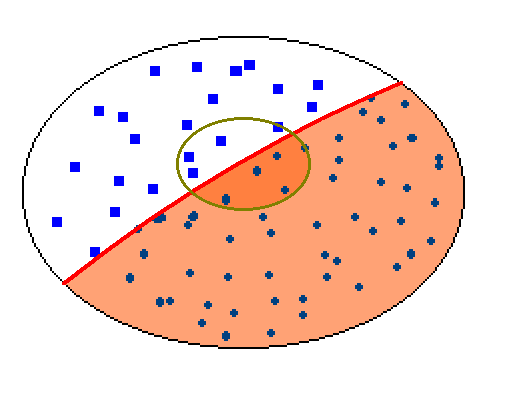
\includegraphics[width=0.5\textwidth,height=\textheight]{figuras/poblacion-muestra.png}
\caption{Población y muestra}
\end{figure}

\(n\) elementos de la muestra
\end{frame}

\begin{frame}{}
\protect\hypertarget{section-2}{}
\begin{block}{Error de muestreo}
\protect\hypertarget{error-de-muestreo}{}
\begin{itemize}
\item
  El error que se comete debido al hecho de que se obtienen conclusiones
  sobre cierta realidad a partir de la observación de sólo una parte de
  ella, se denomina \textbf{error de muestreo}.
\item
  Obtener una muestra adecuada, significa lograr una versión
  simplificada de la población, que reproduzca de algún modo sus rasgos
  y características básicas o de interés.
\end{itemize}
\end{block}
\end{frame}

\begin{frame}{}
\protect\hypertarget{section-3}{}
\begin{block}{Terminología}
\protect\hypertarget{terminologuxeda}{}
\begin{itemize}
\item
  \textbf{Elemento} es un objeto o persona en el cual se toman las
  mediciones.
\item
  \textbf{Población objetivo}: conjunto de individuos de los que se
  quiere obtener información.
\item
  \textbf{Unidades de muestro}: el conjunto de elementos no traslapados
  de la población que cubren a la población completa. Todo miembro de la
  población pertenecerá a una y sólo una unidad de muestreo.
\item
  \textbf{Unidades de análisis}: objeto o individuo del que hay que
  obtener la información.
\item
  \textbf{Marco muestral}: lista de unidades o elementos de muestreo.
\item
  \textbf{Muestra}: conjunto de unidades o elementos de análisis
  seleccionadas de un marco o varios marcos.
\end{itemize}
\end{block}
\end{frame}

\begin{frame}{}
\protect\hypertarget{section-4}{}
\begin{block}{Terminología}
\protect\hypertarget{terminologuxeda-1}{}
\begin{itemize}
\tightlist
\item
  \textbf{Muestreo probabilístico}. El planteamiento clásico del
  problema de estimación estadística requiere que la aleatoriedad esté
  comprendida en el diseño de muestreo para así poder evaluar
  probabilísticamente, las propiedades de los estimadores. Al diseño de
  muestreo que plantea la selección, de unidades de muestreo, basada en
  la aleatoriedad se le llama \emph{muestreo probabilístico}.
\end{itemize}
\end{block}
\end{frame}

\begin{frame}{}
\protect\hypertarget{section-5}{}
\begin{block}{Terminología}
\protect\hypertarget{terminologuxeda-2}{}
\begin{itemize}
\item
  \textbf{Límite para el error de estimación}. Si \(\theta\) es la
  característica poblacional de interés y \(\hat{\theta}\) es un
  estimador (basándose en la información de la muestra) de \(\theta\),
  debemos especificar un límite para el error de estimación; esto es,
  debemos especificar que \(\theta\) y \(\hat{\theta}\) difieran en
  valor absoluto a lo más en cierto valor \(B\). Simbólicamente,
  \[\mbox{error de estimación}=|\theta - \hat{\theta} | < B\]
\item
  \(\theta\) puede ser cualquier característica de la población (el
  promedio, el total, un porcentaje, el valor mediano, el valor mínimo,
  etcétera) Se le llama \textbf{parámetro}.
\item
  \(\hat{\theta}\) es el \textbf{estadístico} obtenido a partir de la
  información de la muestra. En algunas veces llamado estadístico de
  prueba. (el promedio de la muestra, el total de la muestra, el mínimo
  de la muestra, la mediana de la muestra, etcétera)
\end{itemize}
\end{block}
\end{frame}

\begin{frame}{}
\protect\hypertarget{section-6}{}
\begin{block}{Parámetro poblacional vs Estadístico muestral}
\protect\hypertarget{paruxe1metro-poblacional-vs-estaduxedstico-muestral}{}
\begin{itemize}
\tightlist
\item
  \textbf{Parámetro:} Es una cantidad numérica calculada sobre una
  población

  \begin{itemize}
  \tightlist
  \item
    La altura media de los individuos de un país
  \item
    La idea es resumir toda la información que hay en la población en
    unos pocos números (parámetros).
  \end{itemize}
\item
  \textbf{Estadístico:} Es una cantidad numérica calculada sobre una
  muestra de la población

  \begin{itemize}
  \tightlist
  \item
    La altura media de los que estamos en este aula.

    \begin{itemize}
    \tightlist
    \item
      ¿Somos una muestra de la población? ¿representativa?
    \end{itemize}
  \item
    Si un estadístico se usa para aproximar un parámetro también se le
    suele llamar estimador.\footnote<.->{Normalmente nos interesa
      conocer un parámetro, pero por la dificultad que conlleva estudiar
      a \emph{TODA} la población, calculamos un estimador sobre una
      muestra y ``confiamos'' en que sean próximos. Más adelante veremos
      como elegir muestras para que el error sea ``confiablemente''
      pequeño}
  \end{itemize}
\end{itemize}
\end{block}
\end{frame}

\begin{frame}{}
\protect\hypertarget{section-7}{}
\begin{longtable}[]{@{}lll@{}}
\toprule()
& Población & Muestra \\
\midrule()
\endhead
& Parámetro & Estadístico \\
Media & \(\mu\) & \(\bar{x}\) \\
Proporción & \(P\) & \(p\) \\
Máximo & \(max\) & \(max\) \\
Mediana & \(\tilde{x}\) & \\
Varianza & \(\sigma^2\) & \(s^2\) \\
Total & \(T\) & \(\hat{T}\) \\
& \(\theta\) & \(\hat{\theta}\) \\
\bottomrule()
\end{longtable}
\end{frame}

\begin{frame}{}
\protect\hypertarget{section-8}{}
\begin{block}{}
\protect\hypertarget{section-9}{}
\begin{itemize}
\tightlist
\item
  También debemos definir una probabilidad, \((1-\alpha)\) que
  especifique la fracción de veces en muestreo repetido, que
  requeriremos que el error de estimación sea menor que \(B\). Esto es
  \[P[\mbox{error de estimación} < B] = 1 - \alpha\]
\end{itemize}
\end{block}

\begin{block}{}
\protect\hypertarget{section-10}{}
\begin{itemize}
\tightlist
\item
  \textbf{Muestreo no probabilístico}. El muestreo no probabilístico no
  involucra ningún elemento aleatorio en el proceso de selección.
\end{itemize}
\end{block}
\end{frame}

\begin{frame}{}
\protect\hypertarget{section-11}{}
Definición: Si \(X_1, X_2, ..., X_n\) son \textbf{variables aleatorias}
independientes e idénticamente distribuidas, decimos que constituyen una
\textbf{muestra aleatoria} de la población \textbf{infinita} dada por su
distribución común.

Si \(S\) es un espacio muestral con una medida de probabilidad y \(X\)
es una función con valor real definida con respecto a los elementos de
\(S\), entonces \(X\) se denomina \textbf{Variable Aleatoria}.
\end{frame}

\begin{frame}{Muestreo Aleatorio Simple (Población Finita)}
\protect\hypertarget{muestreo-aleatorio-simple-poblaciuxf3n-finita}{}
\begin{block}{}
\protect\hypertarget{section-12}{}
Unas muestra aleatoria simple de tamaño \(n\), de una población finita
de tamaño \(N\), es una muestra seleccionada de tal manera que cada una
de las muestras posibles de tamaño \(n\) tenga la misma probabilidad de
ser seleccionada.
\end{block}
\end{frame}

\begin{frame}{Distribución de Muestreo}
\protect\hypertarget{distribuciuxf3n-de-muestreo}{}
\begin{block}{¿Qué es una distribución muestral?}
\protect\hypertarget{quuxe9-es-una-distribuciuxf3n-muestral}{}
La distribución muestral de un estadístico de prueba proporciona

\begin{enumerate}
\tightlist
\item
  una lista de todos los valores que puede tomar dicho estadístico y
\item
  la probabilidad de obtener cada valor, suponiendo que éste es producto
  sólo del azar.
\end{enumerate}
\end{block}
\end{frame}

\begin{frame}{Distribución muestral de la media}
\protect\hypertarget{distribuciuxf3n-muestral-de-la-media}{}
La distribución muestral de la media proporciona todos los valores que
puede tomar la media, junto con la probabilidad de obtener cada valor si
el muestreo es aleatorio a partir de la población hipotética.

La media muestral posee las siguientes características:

\begin{enumerate}
\item
  \(\mu_{\bar{x}}\)= es la media de la distribución muestral de la
  media.

  \(s_{\bar{x}}\) = es la desviación estándar de la distribución
  muestral de la media
\item
  La media muestral es igual a la media poblacional,
  \(\mu_{\bar{x}}=\mu\).
\item
  La media muestral tiene una desviación estándar igual a la desviación
  estándar poblacional de datos crudos, dividida entre la raíz del
  número de datos. Es decir:
  \(\sigma_{\bar{x}}=\frac{\sigma}{\sqrt{n}}\)
\item
  Presenta una forma de campana.
\end{enumerate}
\end{frame}

\begin{frame}{}
\protect\hypertarget{section-13}{}
A pesar que la demostración de la distribución muestral de la media va
más allá de los alcances del curso, podemos hacer un ejemplo para la
mejor comprensión de la distribución muestral de la media.

Supongamos una población de solo cinco elementos
\(2, 3, 4, 5 \mbox{ y } 6\). La media \(\mu\) de la población es
\(\mu = 4.0\) y la desviación estándar de la población es
\(\sigma = 1.41\).

Ahora queremos deducir la distribución muestral de la media para
muestras de tamaño \(2\) de la población. Extraemos (con reemplazo)
todas las distintas muestras de tamaño \(n = 2\). Y observamos cual es
el valor de \(\bar{x}\) y su probabilidad.
\end{frame}

\begin{frame}{}
\protect\hypertarget{section-14}{}
\begin{table}
\centering\begingroup\fontsize{7}{9}\selectfont

\begin{tabular}{c|c|c|r}
\hline
Var1 & Var2 & promedio & muestra\\
\hline
2 & 2 & 2.0 & 1\\
\hline
3 & 2 & 2.5 & 2\\
\hline
4 & 2 & 3.0 & 3\\
\hline
5 & 2 & 3.5 & 4\\
\hline
6 & 2 & 4.0 & 5\\
\hline
2 & 3 & 2.5 & 6\\
\hline
3 & 3 & 3.0 & 7\\
\hline
4 & 3 & 3.5 & 8\\
\hline
5 & 3 & 4.0 & 9\\
\hline
6 & 3 & 4.5 & 10\\
\hline
2 & 4 & 3.0 & 11\\
\hline
3 & 4 & 3.5 & 12\\
\hline
4 & 4 & 4.0 & 13\\
\hline
5 & 4 & 4.5 & 14\\
\hline
6 & 4 & 5.0 & 15\\
\hline
2 & 5 & 3.5 & 16\\
\hline
3 & 5 & 4.0 & 17\\
\hline
4 & 5 & 4.5 & 18\\
\hline
5 & 5 & 5.0 & 19\\
\hline
6 & 5 & 5.5 & 20\\
\hline
2 & 6 & 4.0 & 21\\
\hline
3 & 6 & 4.5 & 22\\
\hline
4 & 6 & 5.0 & 23\\
\hline
5 & 6 & 5.5 & 24\\
\hline
6 & 6 & 6.0 & 25\\
\hline
\end{tabular}
\endgroup{}
\end{table}
\end{frame}

\begin{frame}{}
\protect\hypertarget{section-15}{}
\begin{minipage}{\textwidth}

\begin{multicols}{2}


\begin{tabular}{c|c|c}
\hline
promedio & conteo & p\\
\hline
2.0 & 1 & 0.04\\
\hline
2.5 & 2 & 0.08\\
\hline
3.0 & 3 & 0.12\\
\hline
3.5 & 4 & 0.16\\
\hline
4.0 & 5 & 0.20\\
\hline
4.5 & 4 & 0.16\\
\hline
5.0 & 3 & 0.12\\
\hline
5.5 & 2 & 0.08\\
\hline
6.0 & 1 & 0.04\\
\hline
\end{tabular}



\begin{flushright}\includegraphics{Distr-muestrales_files/figure-beamer/unnamed-chunk-3-1} \end{flushright}



\end{multicols}

\end{minipage}
\end{frame}

\begin{frame}{}
\protect\hypertarget{section-16}{}
\begin{minipage}{\textwidth}

\begin{multicols}{2}


\begin{table}
\centering\begingroup\fontsize{7}{9}\selectfont

\begin{tabular}{c|c|c|r}
\hline
Var1 & Var2 & promedio & muestra\\
\hline
2 & 2 & 2.0 & 1\\
\hline
3 & 2 & 2.5 & 2\\
\hline
4 & 2 & 3.0 & 3\\
\hline
5 & 2 & 3.5 & 4\\
\hline
6 & 2 & 4.0 & 5\\
\hline
2 & 3 & 2.5 & 6\\
\hline
3 & 3 & 3.0 & 7\\
\hline
4 & 3 & 3.5 & 8\\
\hline
5 & 3 & 4.0 & 9\\
\hline
6 & 3 & 4.5 & 10\\
\hline
2 & 4 & 3.0 & 11\\
\hline
3 & 4 & 3.5 & 12\\
\hline
4 & 4 & 4.0 & 13\\
\hline
5 & 4 & 4.5 & 14\\
\hline
6 & 4 & 5.0 & 15\\
\hline
2 & 5 & 3.5 & 16\\
\hline
3 & 5 & 4.0 & 17\\
\hline
4 & 5 & 4.5 & 18\\
\hline
5 & 5 & 5.0 & 19\\
\hline
6 & 5 & 5.5 & 20\\
\hline
2 & 6 & 4.0 & 21\\
\hline
3 & 6 & 4.5 & 22\\
\hline
4 & 6 & 5.0 & 23\\
\hline
5 & 6 & 5.5 & 24\\
\hline
6 & 6 & 6.0 & 25\\
\hline
\end{tabular}
\endgroup{}
\end{table}

Media de la población
$$\mu = \frac{\sum X}{N} = 4.0$$

Media de la medias muestrales
$$\mu_{\bar{x}}=\frac{\sum \bar{x}}{m}= \frac{100}{25} = 4.0$$
Así, $\mu_{\bar{x}}=\mu$. También del resultado podemos verificar que:
$$\sigma_{\bar{x}}=\frac{\sigma}{\sqrt{n}}=\frac{1.41}{\sqrt{2}}=1.0$$
Pero podemos calcular directamente:

$$\sigma_{\bar{x}}=\sqrt{\frac{\sum (\bar{x}-\mu_{\bar{x}})^2}{m}}=$$ $$=\sqrt{\frac{(2-4)^2 + \cdots \ (6-4)^2}{25}}=1.0$$

\end{multicols}

\end{minipage}
\end{frame}

\begin{frame}{}
\protect\hypertarget{section-17}{}
\begin{block}{Distribución muestral de la media para N=5, con \(\mu=4\),
\(\sigma=\sqrt{2}\) y \(n=2\)}
\protect\hypertarget{distribuciuxf3n-muestral-de-la-media-para-n5-con-mu4-sigmasqrt2-y-n2}{}
\begin{minipage}{\textwidth}

\begin{multicols}{2}


\begin{tabular}{c|c|c}
\hline
promedio & conteo & p\\
\hline
2.0 & 1 & 0.04\\
\hline
2.5 & 2 & 0.08\\
\hline
3.0 & 3 & 0.12\\
\hline
3.5 & 4 & 0.16\\
\hline
4.0 & 5 & 0.20\\
\hline
4.5 & 4 & 0.16\\
\hline
5.0 & 3 & 0.12\\
\hline
5.5 & 2 & 0.08\\
\hline
6.0 & 1 & 0.04\\
\hline
\end{tabular}



\begin{flushright}\includegraphics{Distr-muestrales_files/figure-beamer/unnamed-chunk-6-1} \end{flushright}



\end{multicols}

\end{minipage}
\end{block}
\end{frame}

\begin{frame}{}
\protect\hypertarget{section-18}{}
\begin{block}{Distribución muestral de la media para N=5, con \(\mu=4\),
\(\sigma=\sqrt{2}\) y \(n=3\)}
\protect\hypertarget{distribuciuxf3n-muestral-de-la-media-para-n5-con-mu4-sigmasqrt2-y-n3}{}
\begin{minipage}{\textwidth}

\begin{multicols}{2}


\begin{tabular}{c|c|c}
\hline
promedio & conteo & p\\
\hline
2.000 & 1 & 0.008\\
\hline
2.333 & 3 & 0.024\\
\hline
2.667 & 6 & 0.048\\
\hline
3.000 & 10 & 0.080\\
\hline
3.333 & 15 & 0.120\\
\hline
3.667 & 18 & 0.144\\
\hline
4.000 & 19 & 0.152\\
\hline
4.333 & 18 & 0.144\\
\hline
4.667 & 15 & 0.120\\
\hline
5.000 & 10 & 0.080\\
\hline
5.333 & 6 & 0.048\\
\hline
5.667 & 3 & 0.024\\
\hline
6.000 & 1 & 0.008\\
\hline
\end{tabular}



\begin{flushright}\includegraphics{Distr-muestrales_files/figure-beamer/unnamed-chunk-8-1} \end{flushright}



\end{multicols}

\end{minipage}
\end{block}
\end{frame}

\begin{frame}{}
\protect\hypertarget{section-19}{}
\begin{block}{Distribución muestral de la media para N=5, con \(\mu=4\),
\(\sigma=\sqrt{2}\) y \(n=9\)}
\protect\hypertarget{distribuciuxf3n-muestral-de-la-media-para-n5-con-mu4-sigmasqrt2-y-n9}{}
\begin{center}\includegraphics{Distr-muestrales_files/figure-beamer/unnamed-chunk-9-1} \end{center}

Ver el archivo \textbf{distr\_muestral\_pequena.R} en
\url{https://rstudio.cloud/content/4731243}
\end{block}
\end{frame}

\begin{frame}{Teorema del Límite Central}
\protect\hypertarget{teorema-del-luxedmite-central}{}
\begin{block}{Central Limit Theorem}
\protect\hypertarget{central-limit-theorem}{}
Teorema: Si \(X_1, X_2, \ldots, X_n\) constituyen una muestra aleatoria
de una población infinita que tiene la media \(\mu\) y la varianza
\(\sigma^2\), entonces la distribución límite de:
\[\bar{x} \sim N\left(\mu_{\bar{x}}=\mu,\sigma_{\bar{x}}=\frac{\sigma}{\sqrt{n}}\right)\]

cuando \(n \to \infty\). Si definimos

\[Z=\frac{\bar{x}-\mu}{{\sigma}/{\sqrt{n}}}\]

entonces \(Z \sim N(0,1)\) (la distribución normal estándar).
\end{block}

\begin{block}{}
\protect\hypertarget{section-20}{}
Una forma sencilla de expresar el teorema del límite central es: ``la
suma (o promedio) de \(n\) variables aleatorias independientes e
idénticamente distribuidas (\(i.i.d.\)), sigue una distribución límite
normal con media \(n\mu\) (ó \(\mu\)) y varianza \(\sigma^2\)
(\(\sigma^2 /n\))''.
\end{block}
\end{frame}

\begin{frame}{}
\protect\hypertarget{section-21}{}
\begin{block}{Ejemplo}
\protect\hypertarget{ejemplo}{}
Una maquina vendedora de refrescos está programada para que la cantidad
de refresco que se sirva sea una variable aleatoria con una media de
\(200\) mililitros y una desviación estándar de \(15\) mililitros. ¿cuál
es la probabilidad de que la cantidad de refresco promedio (media)
servida en una muestra tomada al azar de \(36\), sea cuando menos
\(204\) mililitros.

\textbf{Solución}

Según el TLC, la distribución de \(\bar{x}\) tiene la media
\(\mu_{\bar{x}}=200\) y desviación estándar
\(s_{\bar{x}}=15/\sqrt{36}= 2.5\), y tiene una distribución que es
aproximadamente normal. Como \(z =(204 -200)/2.5 = 1.6\), podemos
calcular la probabilidad \(P(\bar{x} \ge 204) = P(z \ge 1.6) = 0.0548\).
\end{block}
\end{frame}

\begin{frame}{}
\protect\hypertarget{section-22}{}
Para que se alcance una distribución parecida a la normal en el conjunto
de posibles promedios muestrales se requiere que \(n\) sea grande.

Sin embargo, la rapidez de acercamiento a la normal (velocidad de
convergencia) también depende de la forma de la distribución de la
variable en la población.

Ver la siguiente liga de de una aplicación hecha en shinny donde se
puede ver el histograma de promedios, donde sepuede modificar el número
de simulaciones y el tamaño de la muestra \(n\) de cuatro distribuciones
distintas.

\url{https://s3rgionava.shinyapps.io/histograma_de_medias/}
\end{frame}

\begin{frame}{Distribución de la media (población finita)}
\protect\hypertarget{distribuciuxf3n-de-la-media-poblaciuxf3n-finita}{}
Si \(\bar{x}\) es la media de una muestra aleatoria de tamaño \(n\)
tomada de una población finita de tamaño \(N\) con media \(\mu\) y la
varianza \(\sigma^2\), entonces:
\[E(\bar{x})=\mu \mbox{ y } Var(\bar{x})=\frac{\sigma^2}{n}\cdot\frac{N-n}{N-1}\]
\end{frame}

\begin{frame}{Distribución muestral de proporciones.}
\protect\hypertarget{distribuciuxf3n-muestral-de-proporciones.}{}
\begin{block}{Distribución Binomial}
\protect\hypertarget{distribuciuxf3n-binomial}{}
\textbf{Definición}: Si \(X_1, X_2, \ldots, X_n\) son variables
aleatorias independientes e idénticamente distribuidas (\(i.i.d.\)) que
solo toman valores de \(X_i = 1\) ó \(X_i = 0\), dependiendo si poseen o
no la característica de interés respectivamente, decimos que constituyen
una \textbf{muestra aleatoria de un experimento binomial} de la
población infinita dada por su distribución común.

\textbf{Definición}: Si \(X_1, X_2, \ldots, X_n\) constituyen una
muestra aleatoria de un experimento binomial, entonces
\[p=\frac{\sum_{i=1}^{n}x_i}{n}\] se denomina \textbf{proporción de la
muestra} y \[np(1-p)\] es la \textbf{varianza de la muestra}.
\end{block}
\end{frame}

\begin{frame}{}
\protect\hypertarget{section-23}{}
\begin{figure}
\centering
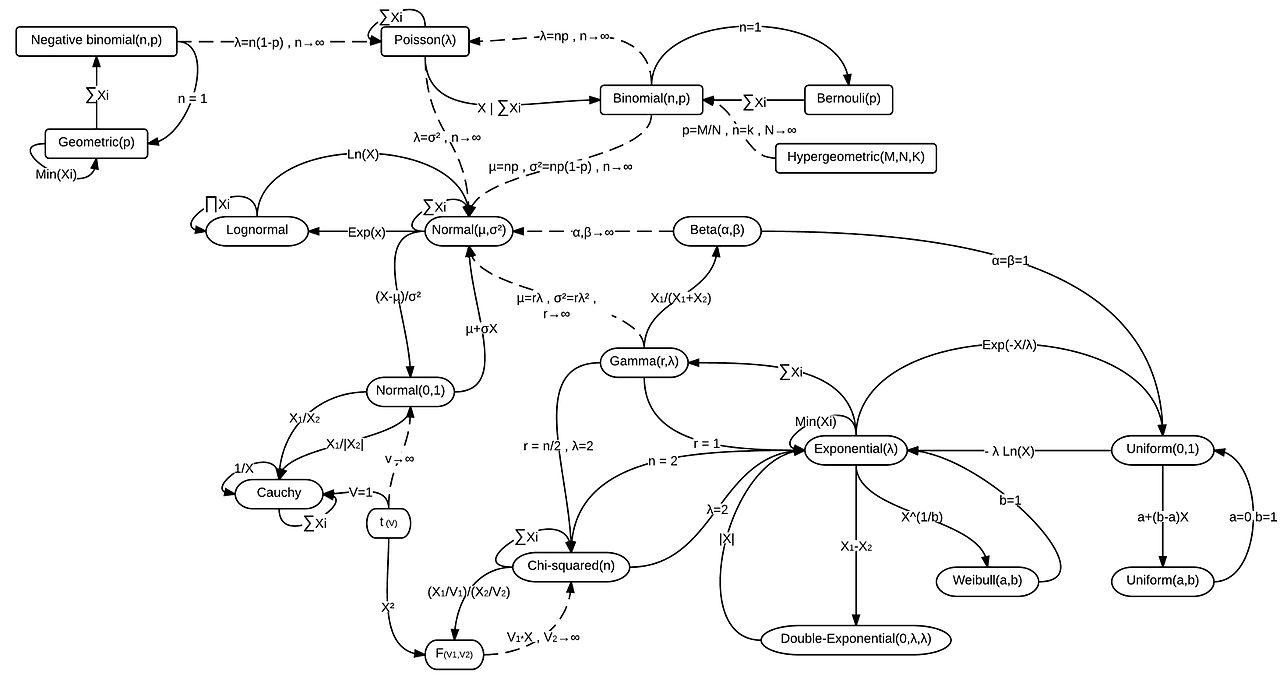
\includegraphics[width=1\textwidth,height=\textheight]{figuras/1280px-Relationships_among_some_of_univariate_probability_distributions.jpg}
\caption{Relaciones entre distribuciones de probabilidad}
\end{figure}

\href{https://en.wikipedia.org/wiki/Relationships_among_probability_distributions\#/media/File:Relationships_among_some_of_univariate_probability_distributions.jpg}{Para
verlo a detalle hacer clic aquí}
\end{frame}

\begin{frame}{}
\protect\hypertarget{section-24}{}
\begin{block}{Para un tamaño de muestra suficientemente grande}
\protect\hypertarget{para-un-tamauxf1o-de-muestra-suficientemente-grande}{}
\textbf{Teorema}: Si \(X_1, X_2, \ldots, X_n\) constituyen una muestra
aleatoria de una población infinita donde \(X_i\) constituye un
experimento Bernoulli, tal que que \(P\) es la proporción de la
población con la característica de interés, entonces se cumple que:
\[E(p)=P \mbox{ y } Var(p)=\frac{p(1-p)}{n}\] \textbf{Corolario}: De
aquí y del TLC se tiene que la distribución límite de
\[z=\frac{p-P}{\sqrt{\frac{p(1-p)}{n}}}\] cuando \(n \to \infty\) es
normal estándar.
\end{block}
\end{frame}

\begin{frame}{}
\protect\hypertarget{section-25}{}
\textbf{Ejemplo}

La proporción de familias de la ciudad de Aguascalientes, que son dueñas
(no arrendatarias) de sus casas es de \(0.70\). Si al azar se
entrevistan a \(84\) familias de esta ciudad y sus respectivas
respuestas (a la pregunta de si son dueñas o no de su casa) se
consideran valores de variables aleatorias independientes que tienen
distribución de Bernoulli idénticas con el parámetro \(P = 0.70\), ¿Con
qué probabilidad podemos afirmar que el valor que se obtenga de la
muestra \(p\) será menor que \(0.64\)

\textbf{Respuesta}

\(P = 0.70\), \(p = 0.64\), \(n = 84\), sustituyendo
\[z=\frac{p-P}{\sqrt{\frac{p(1-p)}{n}}}=\frac{0.64-0.70}{\sqrt{\frac{0.64(0.36)}{84}}}= -1.1456\]

\[p(x<64)=p(z< -1.1456)=0.1259\]
\end{frame}

\begin{frame}{}
\protect\hypertarget{section-26}{}
\begin{block}{Aproximación para proporciones}
\protect\hypertarget{aproximaciuxf3n-para-proporciones}{}
También se puede ver este resultado como dada una muestra aleatoria
\(X_1, X_2, \ldots, X_n\) de variables aleatorias Bernoulli, con
\(x =\sum_{i=1}^n x_i\) el número de éxitos observados, en \(n\)
intentos igualmente probables, entonces la distribución límite de:
\[z=\frac{x-np}{\sqrt{n p (1-p)}}\] con \(p=x/n\), para
\(n \to \infty\), \(z\) tiene una distribución límite normal estándar.
\end{block}
\end{frame}

\begin{frame}{Distribución t-Student (William S. Gosset)}
\protect\hypertarget{distribuciuxf3n-t-student-william-s.-gosset}{}
\begin{block}{}
\protect\hypertarget{section-27}{}
Si \(\bar{x}\) y \(s^2\) son la media y la varianza de una muestra
aleatoria de tamaño \(n\) tomada de una población \textbf{normal} con
media \(\mu\) , entonces \[t=\frac{\bar{x}-\mu}{s/\sqrt{n}}\]

tiene una distribución \emph{t-student} con \(n-1\) grados de libertad.

Para usar la distribución normal es necesario conocer el valor de la
desviación estandar poblacional \(\sigma\). Como es más común el
desconocimiento, entonces se estima \(\sigma\) a través de \(s\)
(desviación estándar muestral) y se usa la distribución \(t\).

\[z=\frac{\bar{x}-\mu}{\sigma /\sqrt{n}}\]
\end{block}
\end{frame}

\begin{frame}{}
\protect\hypertarget{section-28}{}
\begin{center}\includegraphics{Distr-muestrales_files/figure-beamer/unnamed-chunk-10-1} \end{center}
\end{frame}

\begin{frame}{}
\protect\hypertarget{section-29}{}
\begin{block}{Teorema}
\protect\hypertarget{teorema}{}
Sea \(Z\) una variable aleatoria normal estándar y \(V\) una variable
aleatoria chi cuadrada con \(\nu\) grados de libertad. Si \(Z\) y \(V\)
son independientes, entonces la distribución de la variable aleatoria
\(T\), donde \[T=\frac{Z}{\sqrt{V/\nu}}\] está dada por la función de
densidad
\[h(t)=\frac{\Gamma[(\nu+1)/2]}{\Gamma(\nu/2)\sqrt{\pi \nu}}\left(1+\frac{t^2}{\nu}\right)^{-(\nu +1)/2}\quad , -\infty <t<\infty\]
Ésta distribución se conoce como \textbf{distribución t} con \(\nu\)
grados de libertad.
\end{block}
\end{frame}

\begin{frame}{}
\protect\hypertarget{section-30}{}
\begin{block}{Corolario}
\protect\hypertarget{corolario}{}
Sean \(X_1, X_2,\cdots, X_n\) variables aleatorias independientes norma
les con media \(\mu\) y desviación estándar \(\sigma\). Sea
\[\bar{X}=\frac{1}{n}\sum_{i=1}^n X_i \qquad\mbox{ y } \qquad S^2=\frac{1}{n-1}\sum_{i=1}^n (X_i-\bar{X})^2.\]
Entonces la variable aleatoria \(\frac{\bar{x}-\mu}{s/\sqrt{n}}\) tiene
una distribución \(t\) con \(\nu=n-1\) grados de libertad.
\end{block}
\end{frame}

\begin{frame}{}
\protect\hypertarget{section-31}{}
\begin{block}{Ejemplo}
\protect\hypertarget{ejemplo-1}{}
Suponga que usted tiene una técnica que puede modificar la edad a la
cual los niños empiezan a hablar. En su localidad, el promedio de edad,
en la cual un niño emite su primera palabra, es \(13\) meses. No conoce
la desviación estandar poblacional. Usted aplica dicha técnica a una
muestra de \(15\) niños. Los resultados son los
siguientes:\(8, 9, 10, 15, 18, 17, 12, 11, 7, 8, 10, 11, 8, 9, 12\).
\(n = 15\), \(\bar{x} = 11.0\), desviación estándar \(s = 3.34\). Si la
media poblacional (verdadera) es \(13\) meses, ¿cuál es la probabilidad
de encontrar un valor igual o menor de \(\bar{x}\) de \(11\) meses?

\textbf{Solución}

Se tiene que \(\mu =13\), \(s=3.34\), \(\bar{x}=11\) y \(n=15\).
Sustituyendo se obtiene

\[t=\frac{\bar{x}-\mu}{s/\sqrt{n}}=\frac{11-13}{3.34/\sqrt{15}}=-2.32\]
Por lo tanto \(P(\bar{x}\le 11)=P(t \le -2.32) =\) 0.0179795.
\end{block}
\end{frame}

\begin{frame}{}
\protect\hypertarget{section-32}{}
\begin{center}\includegraphics{Distr-muestrales_files/figure-beamer/unnamed-chunk-11-1} \end{center}
\end{frame}

\begin{frame}{}
\protect\hypertarget{section-33}{}
\begin{figure}
\centering
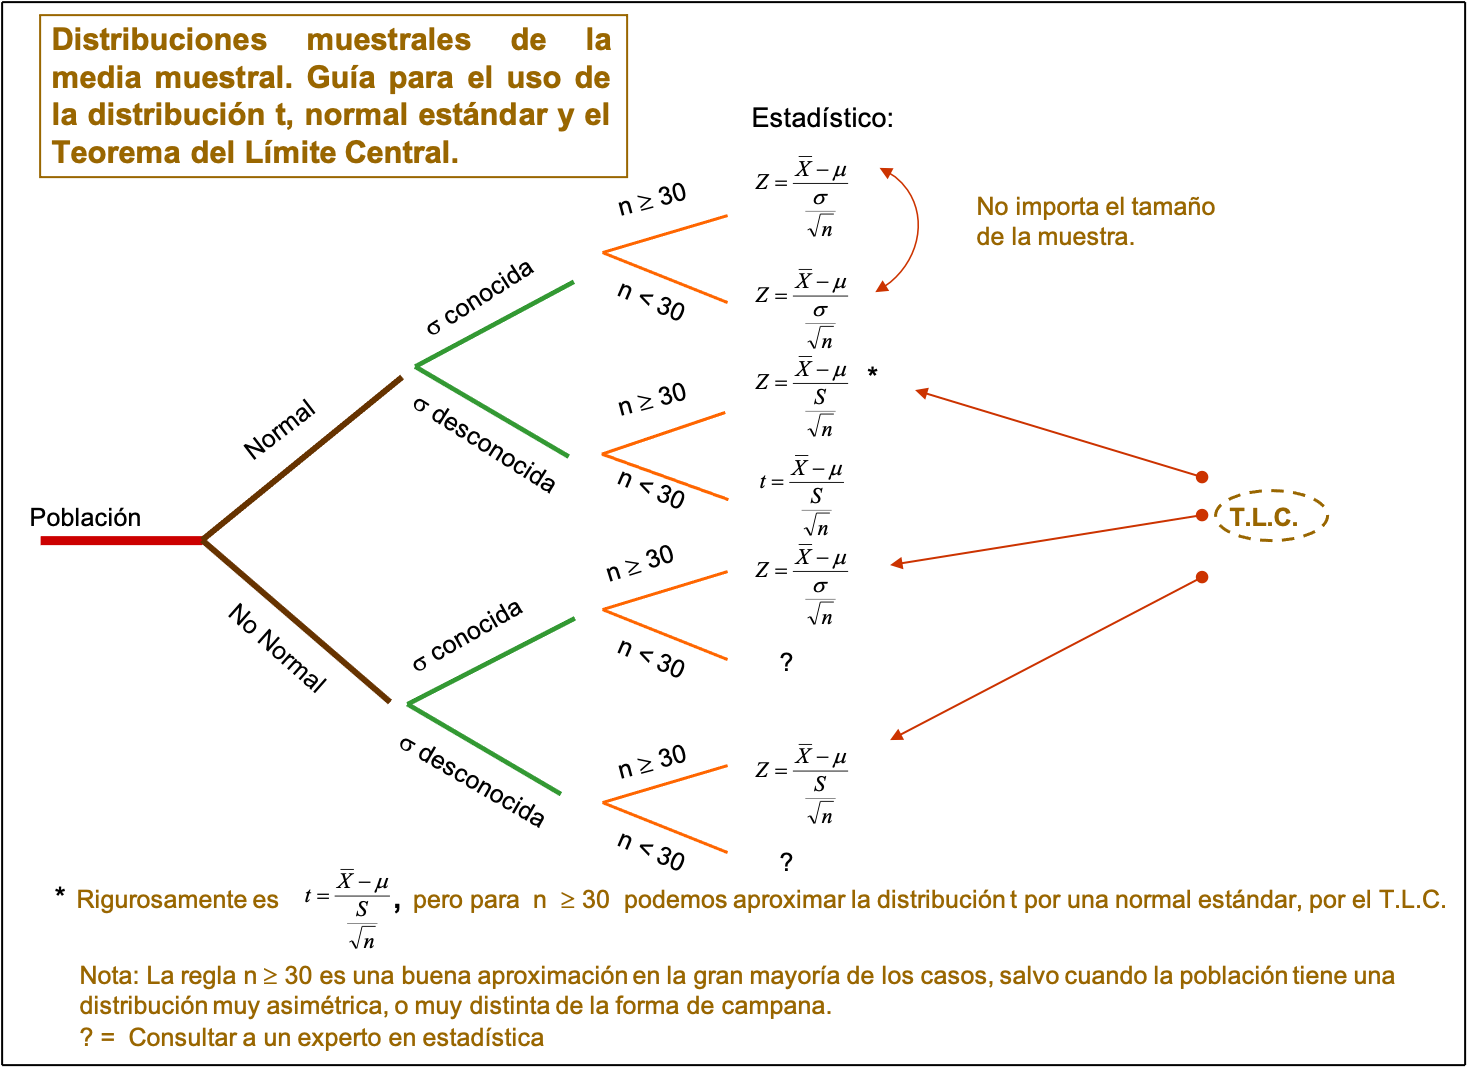
\includegraphics[width=0.9\textwidth,height=\textheight]{figuras/dist-muest-media.png}
\caption{Distribuciones muestrales de la media}
\end{figure}
\end{frame}

\begin{frame}{Distribución normal y las poblaciones discretas.}
\protect\hypertarget{distribuciuxf3n-normal-y-las-poblaciones-discretas.}{}
\textbf{Aplicaciones}

La distribución de normal se emplea muchas veces como una aproximación
de valores en una población discreta. En situaciones, debe tenrse
especial cuidado para asegurar que las probabilidades se calculan de
manera precisa.

Considérese el siguiente ejemplo: Se sabe que el Coeficiente de
Inteligencia (CI) de una población está distribuido normalmente en forma
aproximada con \(\mu =100\) y \(\sigma = 15\). ¿Cuál es la probabilidad
de que un individuo seleccionado al azar tenga un CI de por lo menos
125? Si se hace \(X = IC\) de una persona elegida al azar, deseamos
\(P(X \ge 125)\).

La tentación aquí es estandarizar como en los ejemplos anteriores. Sin
embargo, la población del CI es discreta en realidad, ya que los CI son
de valor entero, y la curva normal es una aproximación a un histograma
de probabilidad discreta.
\end{frame}

\begin{frame}{}
\protect\hypertarget{section-34}{}
Los rectángulos del histograma están centrados como enteros, y los CI de
por lo menos 125 corresponden a rectángulos que se inician en 124.5. En
realidad deseamos \(P(X \ge 124.5)\), que ahora se puede estandarizar
para obtener \(P(Z \ge 1.63) = 0.0516\).

Si hubieramos estandarizado \(X \ge 125\), habríamos obtenido
\(P(Z \ge 1.67) = 0.0475\). La diferencia no es grande, pero la
respuesta \(0.0516\) es más precisa. Análogamente, \(P(X = 125)\) sería
más apropiado por el área entre \(124.5\) y \(125.5\). Ya que el área
bajo la curva normal arriba del valor único de \(125\) es cero.

La corrección para la discretización de la distribución subyacente se
llama con frecuencia \textbf{corrección de continuidad}. Es útil en la
siguiente aplicación de la distribución normal
\end{frame}

\begin{frame}{Aproximación de la distribución binomial a la distribución
normal.}
\protect\hypertarget{aproximaciuxf3n-de-la-distribuciuxf3n-binomial-a-la-distribuciuxf3n-normal.}{}
Recordemos que el valor medio y la desviación estándar de una variable
aleatoria \(X\) binomial son \(\mu_X = np\) \(\sigma_X = \sqrt{npq}\),
respectivamente. El siguiente histograma muestra una distribución
binomial con \(n = 20\), \(p = 0.6\) (así que \(\mu = 12\),
\(\sigma = [20(0.6)(0.4)]^{1/2} = 2.19\)).

\begin{center}\includegraphics{Distr-muestrales_files/figure-beamer/unnamed-chunk-12-1} \end{center}
\end{frame}

\begin{frame}{}
\protect\hypertarget{section-35}{}
Una curva normal con valor medio y desviación estándar igual a los
valores correspondientes para la distribución binomial se ha sobrepuesto
en el histograma de probabilidad. Aun cuando el histograma esta un poco
sesgado (porque \(p \ne 0.5\)), la curva normal da una buena
aproximación, en especial en la parte media de la figura.

\begin{center}\includegraphics{Distr-muestrales_files/figure-beamer/unnamed-chunk-13-1} \end{center}
\end{frame}

\begin{frame}{}
\protect\hypertarget{section-36}{}
\begin{minipage}{\textwidth}

\begin{multicols}{2}


\begin{table}
\centering\begingroup\fontsize{9}{11}\selectfont

\begin{tabular}{c|c|c}
\hline
x & Binomial & Normal\\
\hline
0 & 0.000 & 0.000\\
\hline
1 & 0.000 & 0.000\\
\hline
2 & 0.000 & 0.000\\
\hline
3 & 0.000 & 0.000\\
\hline
4 & 0.000 & 0.000\\
\hline
5 & 0.001 & 0.001\\
\hline
6 & 0.005 & 0.005\\
\hline
7 & 0.015 & 0.014\\
\hline
8 & 0.035 & 0.035\\
\hline
9 & 0.071 & 0.072\\
\hline
10 & 0.117 & 0.120\\
\hline
11 & 0.160 & 0.163\\
\hline
12 & 0.180 & 0.181\\
\hline
13 & 0.166 & 0.163\\
\hline
14 & 0.124 & 0.120\\
\hline
15 & 0.075 & 0.072\\
\hline
16 & 0.035 & 0.035\\
\hline
17 & 0.012 & 0.014\\
\hline
18 & 0.003 & 0.005\\
\hline
19 & 0.000 & 0.001\\
\hline
20 & 0.000 & 0.000\\
\hline
\end{tabular}
\endgroup{}
\end{table}

Para el caso binomial: Tenemos que $X\sim Binom(n,p)$
$$P(X=x;n,p)= \binom{n}{x}p^x (1-p)^{n-x}.$$
Si definimos $\mu=np$, $\sigma=\sqrt{np(1-p)}$, podemos aproximar a $X$ mediante la variable $Y\sim N(\mu,\sigma)$ si calculamos de la siguiente forma:
$$P(X=x) \approx P(x-.5 \le Y \le x+.5)$$
$$=P\left(\frac{[x-.5] - \mu}{\sigma} \le Z\le \frac{[x+.5]- \mu}{\sigma}\right)$$



\end{multicols}

\end{minipage}
\end{frame}

\begin{frame}{}
\protect\hypertarget{section-37}{}
El área de cualquier rectángulo (probabilidad de cualquier valor de
\(X\) particular), excepto los de las colas de los extremos, se puede
aproximar con presición mediante el área de la curva normal
correspondiente.

Por ejemplo, \(P(X = 10) = b(X=10; n =20, p = 0.6) = 0.117\), mientras
que el área bajo la curva normal entre \(9.5\) y \(10.5\) es
\(P(-1.14 < Z < -0.68) = 0.120\).

Más generalmente, mientras el histograma de probabilidad binomial no
esté demasiado sesgado, las probabilidades binomiales se pueden
aproximar bien por áreas de curva normal. Se dice entonces que \(X\)
tiene aproximadamente una distribución normal.
\end{frame}

\begin{frame}{}
\protect\hypertarget{section-38}{}
\textbf{Proposición} : Sea \(X\) una V.A. Binomial basada en \(n\)
intentos con probabilidad de éxito \(p\). Entonces, si el histograma de
probabilidad binomial no está demasiado sesgado, \(X\) tiene
aproximadamente una distribución normal con \(\mu = np\) y
\(\sigma = \sqrt{npq}\).

En particular, para \(x =\) un valor posible de \(X\),
\(P(X \le x) = B(x;n,p) \approx\) (área bajo la curva normal estándar a
la izquierda de \(x + 0.5\)), es decir

\[P(X \le x) = B(x;n,p)  \approx \Phi \left( \frac{x+0.5-np}{\sqrt{np(1-p)}}\right)\]

En la práctica la aproximación es adecuada si \(np \ge 5\) y
\(n(1-p) \ge 5\).
\end{frame}

\begin{frame}{Papel De Probabilidad Normal}
\protect\hypertarget{papel-de-probabilidad-normal}{}
La gráfica de papel de Probabilidad Normal, o simplemente gráfica de
probabilidad normal, es un procedimiento útil para verificar si un
conjunto de datos puede ser adecuadamente modelado por una distribución
normal (Bondad de Ajuste). Este procedimiento consiste en construir una
gráfica en el plano cartesiano, en donde, \emph{en el eje horizontal se
grafican los datos} y \emph{en el eje vertical la probabilidad empírica
(acumulada)} de los datos sobre una \emph{escala de probabilidad
normal}.

Es decir, es una gráfica que representa la distribución normal acumulada
de los datos sobre una escala de probabilidad normal. Para construir la
gráfica de probabilidad normal, deben disponerse los datos en orden
ascendente y dibujar el \(k-ésimo\) de estos datos ordenados contra su
punto de probabilidad acumulada \(Pk = (k - 1/2)/n\) sobre papel de
probabilidad normal. Si la distribución de los datos es normal, esta
gráfica deberá parecer una línea recta.
\end{frame}

\begin{frame}{}
\protect\hypertarget{section-39}{}
\begin{minipage}{\textwidth}

\begin{multicols}{2}

Para ejemplificar, considere los $n=25$ datos siguientes.

\begin{table}
\centering\begingroup\fontsize{9}{11}\selectfont

\begin{tabular}{c|c|c|c|c}
\hline
-0.8 & 3.4 & -2.8 & -2.6 & 1.2\\
\hline
2.6 & 0.4 & 0.2 & 5.2 & 1.4\\
\hline
-3.4 & 0.4 & 0.2 & -0.8 & 1.6\\
\hline
-2.8 & -3.8 & -3.4 & -2.6 & 2.6\\
\hline
1.4 & 1.4 & 0.4 & 4.2 & -3.6\\
\hline
\end{tabular}
\endgroup{}
\end{table}

Ahora procederemos a ordenar de menor a mayor y calculamos el valor de $P_k$ para el $k-ésimo$ valor ordenado correspondiente con la expresión

$$P_k = \frac{(k - 1/2)}{n}$$



\begin{table}
\centering\begingroup\fontsize{7}{9}\selectfont

\begin{tabular}{c|c|c|c}
\hline
k & x & Pk & Porcentaje\\
\hline
1 & -3.8 & 0.02 & 2\\
\hline
2 & -3.6 & 0.06 & 6\\
\hline
3 & -3.4 & 0.10 & 10\\
\hline
4 & -3.4 & 0.14 & 14\\
\hline
5 & -2.8 & 0.18 & 18\\
\hline
6 & -2.8 & 0.22 & 22\\
\hline
7 & -2.6 & 0.26 & 26\\
\hline
8 & -2.6 & 0.30 & 30\\
\hline
9 & -0.8 & 0.34 & 34\\
\hline
10 & -0.8 & 0.38 & 38\\
\hline
11 & 0.2 & 0.42 & 42\\
\hline
12 & 0.2 & 0.46 & 46\\
\hline
13 & 0.4 & 0.50 & 50\\
\hline
14 & 0.4 & 0.54 & 54\\
\hline
15 & 0.4 & 0.58 & 58\\
\hline
16 & 1.2 & 0.62 & 62\\
\hline
17 & 1.4 & 0.66 & 66\\
\hline
18 & 1.4 & 0.70 & 70\\
\hline
19 & 1.4 & 0.74 & 74\\
\hline
20 & 1.6 & 0.78 & 78\\
\hline
21 & 2.6 & 0.82 & 82\\
\hline
22 & 2.6 & 0.86 & 86\\
\hline
23 & 3.4 & 0.90 & 90\\
\hline
24 & 4.2 & 0.94 & 94\\
\hline
25 & 5.2 & 0.98 & 98\\
\hline
\end{tabular}
\endgroup{}
\end{table}




\end{multicols}

\end{minipage}
\end{frame}

\begin{frame}{}
\protect\hypertarget{section-40}{}
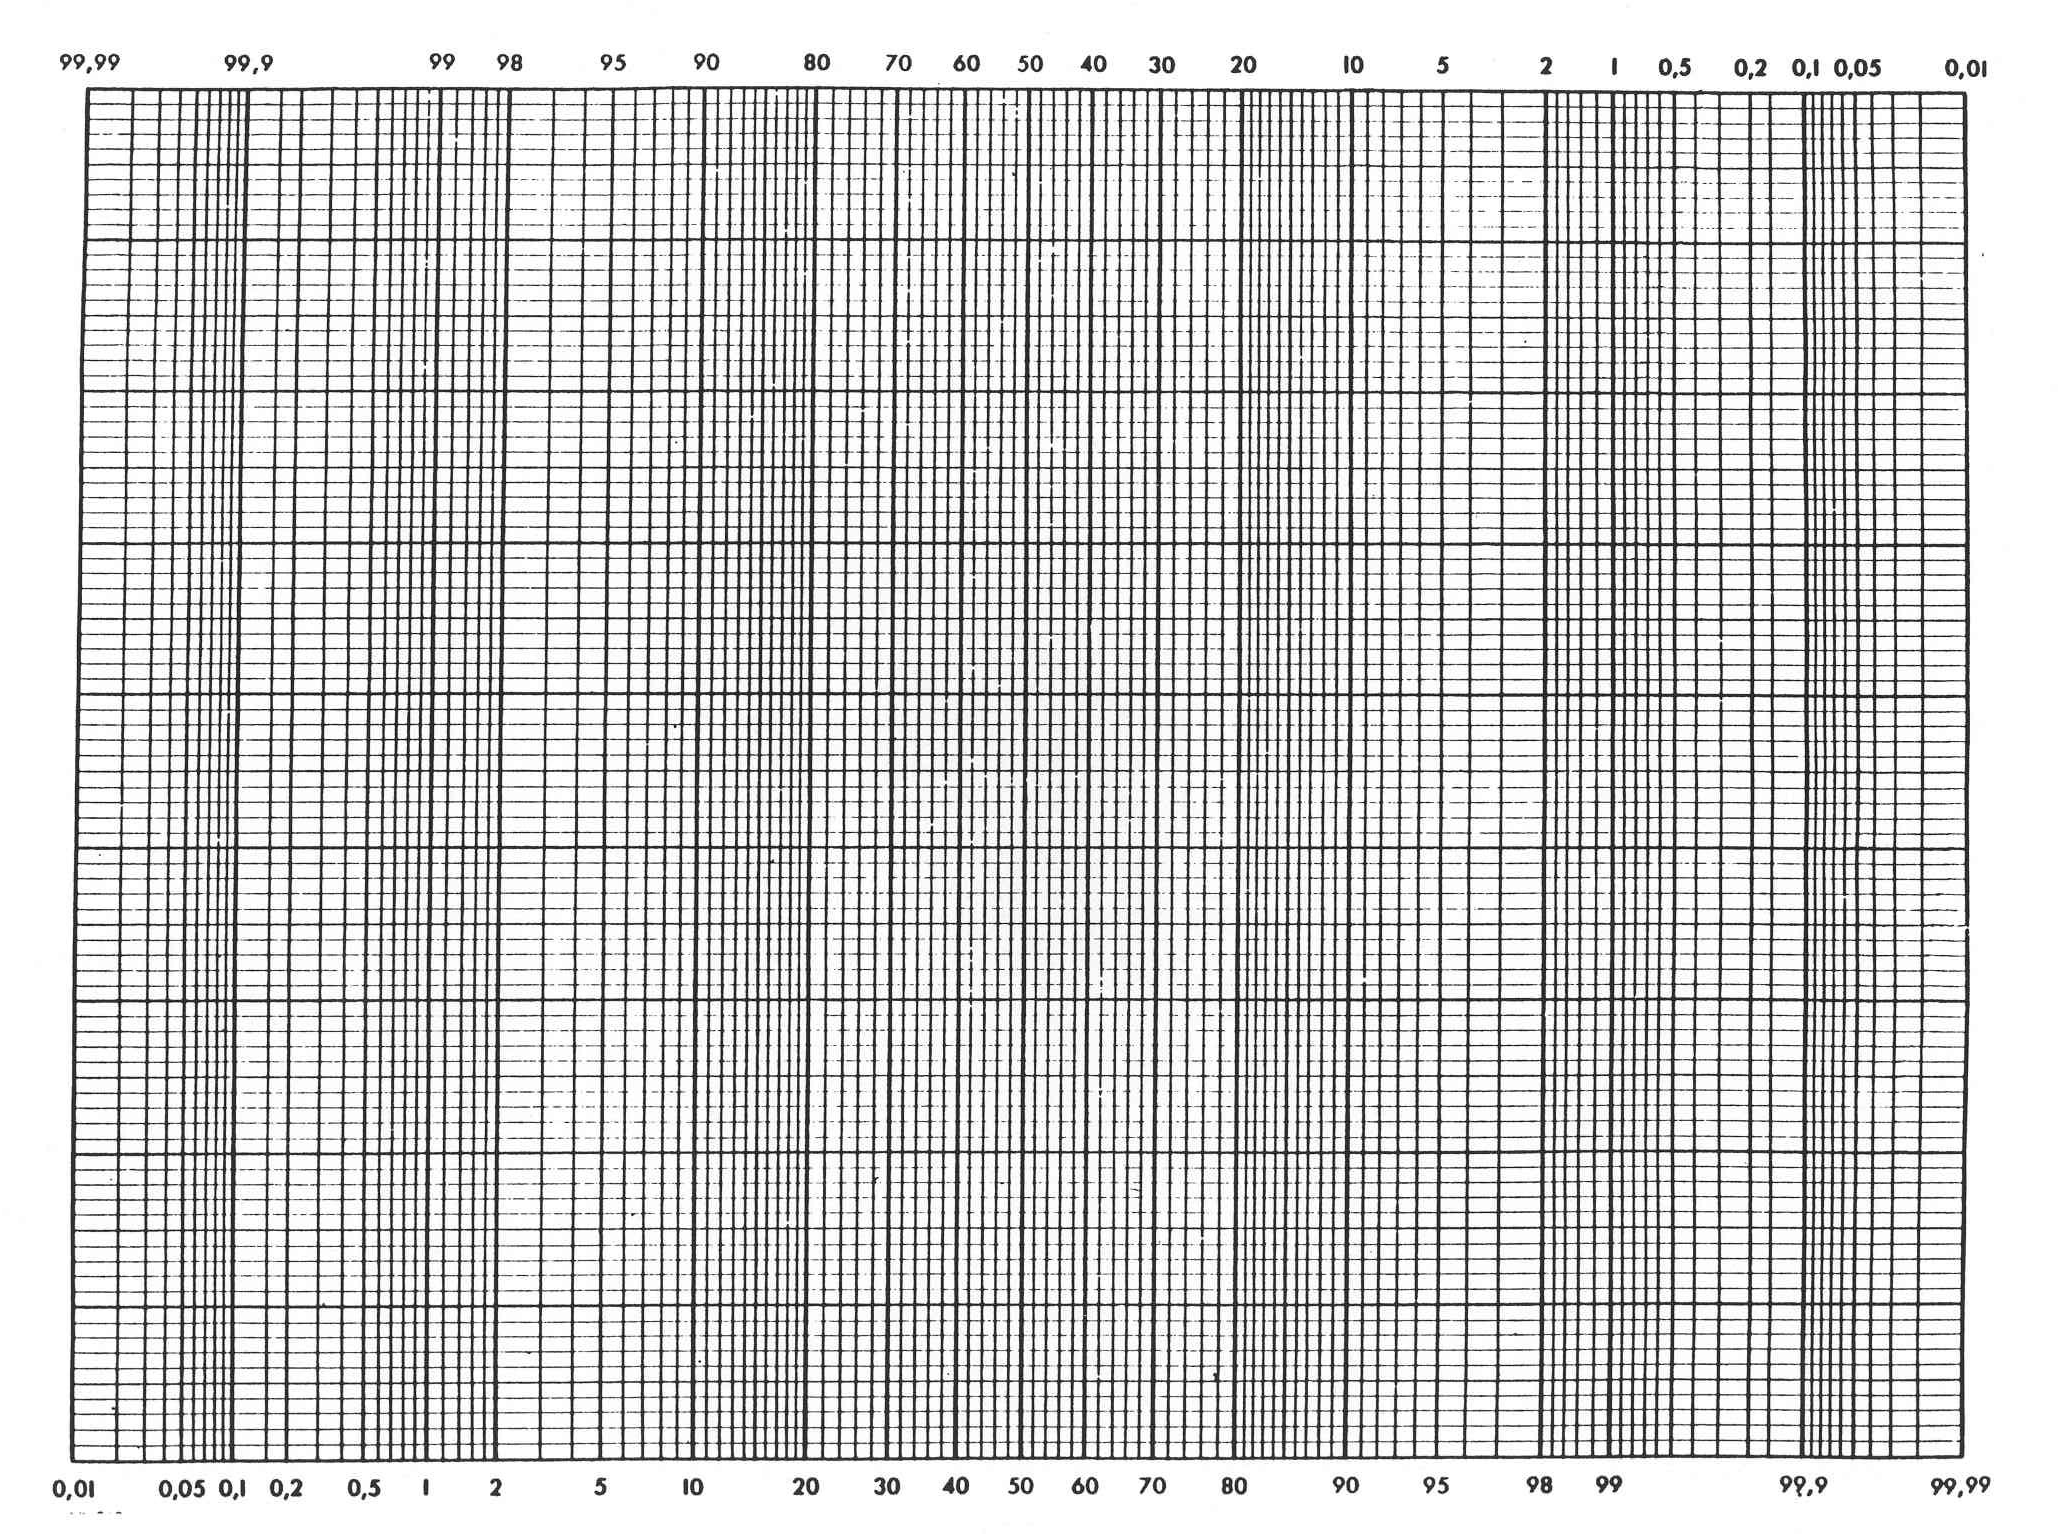
\includegraphics{figuras/probpaperLandscape.png}
\end{frame}

\begin{frame}{}
\protect\hypertarget{section-41}{}
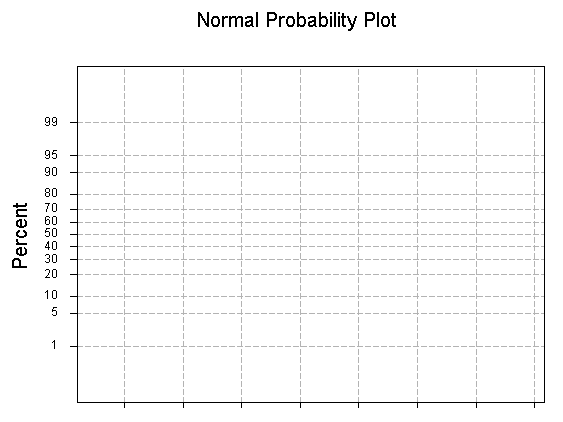
\includegraphics[width=2\textwidth,height=\textheight]{figuras/probpaperLandscape2.png}
\end{frame}

\begin{frame}{}
\protect\hypertarget{section-42}{}
\begin{center}\includegraphics{Distr-muestrales_files/figure-beamer/unnamed-chunk-17-1} \end{center}
\end{frame}

\begin{frame}{}
\protect\hypertarget{section-43}{}
\begin{longtable}[]{@{}
  >{\raggedright\arraybackslash}p{(\columnwidth - 2\tabcolsep) * \real{0.5333}}
  >{\raggedleft\arraybackslash}p{(\columnwidth - 2\tabcolsep) * \real{0.4667}}@{}}
\toprule()
\endhead
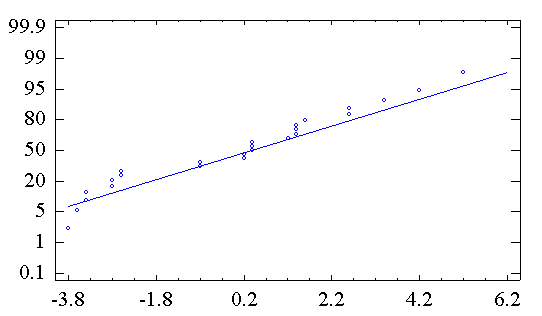
\includegraphics[width=0.45\textwidth,height=\textheight]{figuras/Papel1.png}
&
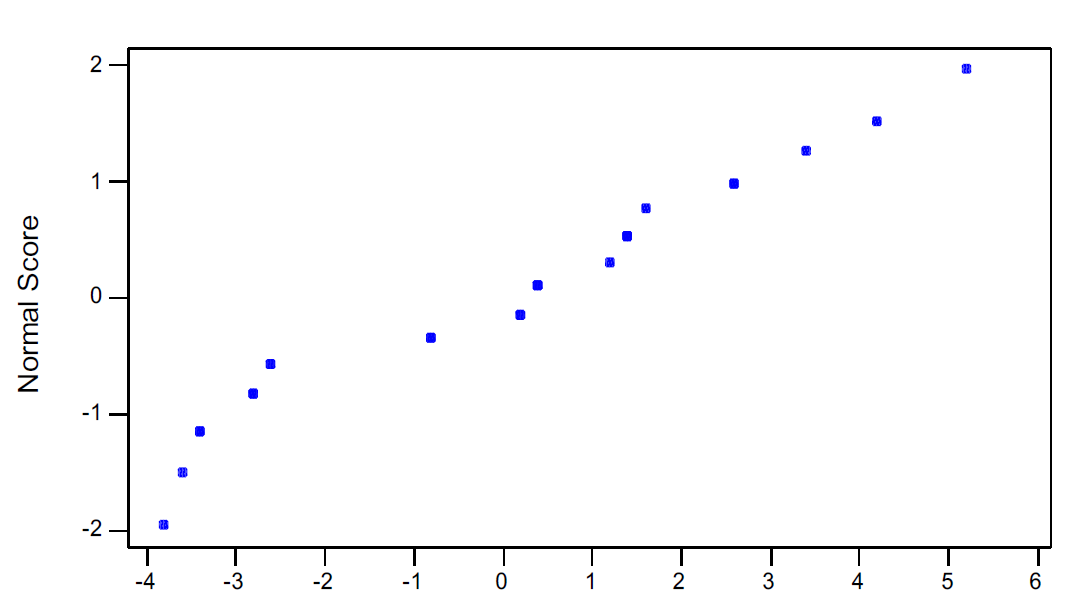
\includegraphics[width=0.45\textwidth,height=\textheight]{figuras/Papel2.png} \\
\bottomrule()
\end{longtable}
\end{frame}

\begin{frame}{}
\protect\hypertarget{section-44}{}
\begin{longtable}[]{@{}
  >{\raggedleft\arraybackslash}p{(\columnwidth - 2\tabcolsep) * \real{0.5333}}
  >{\raggedright\arraybackslash}p{(\columnwidth - 2\tabcolsep) * \real{0.4667}}@{}}
\toprule()
\endhead
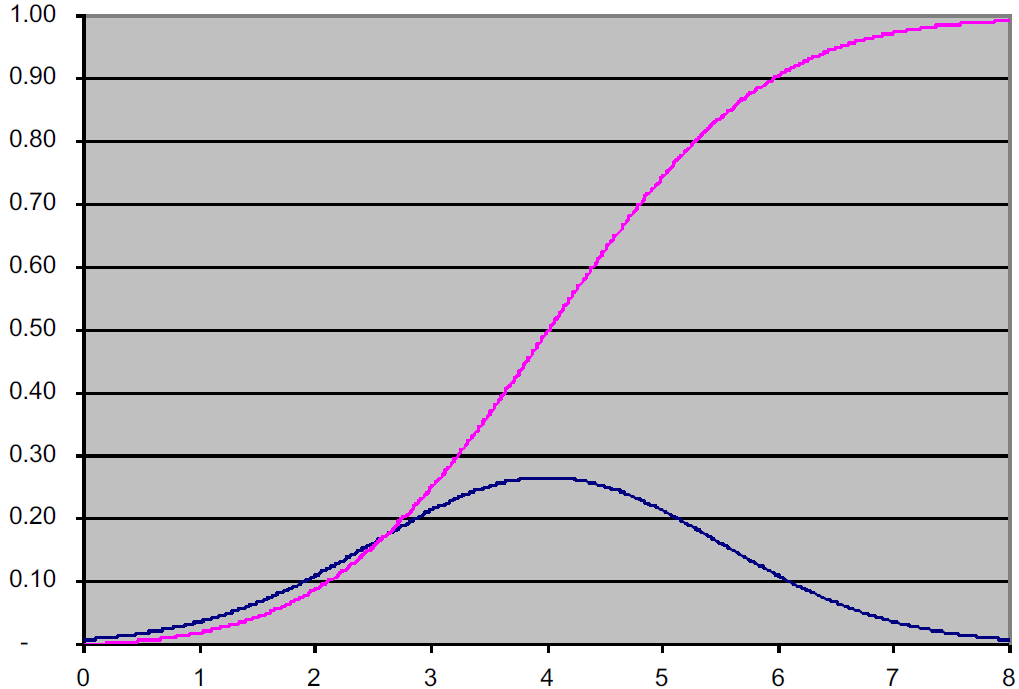
\includegraphics[width=0.45\textwidth,height=\textheight]{figuras/Papel3.png}
&
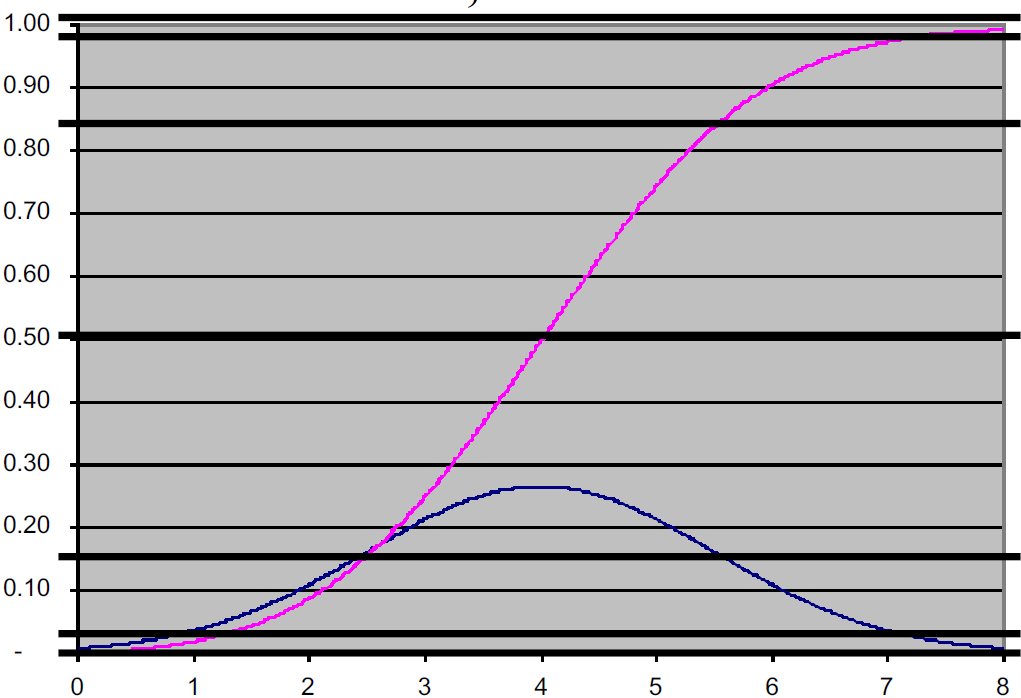
\includegraphics[width=0.45\textwidth,height=\textheight]{figuras/Papel4.png} \\
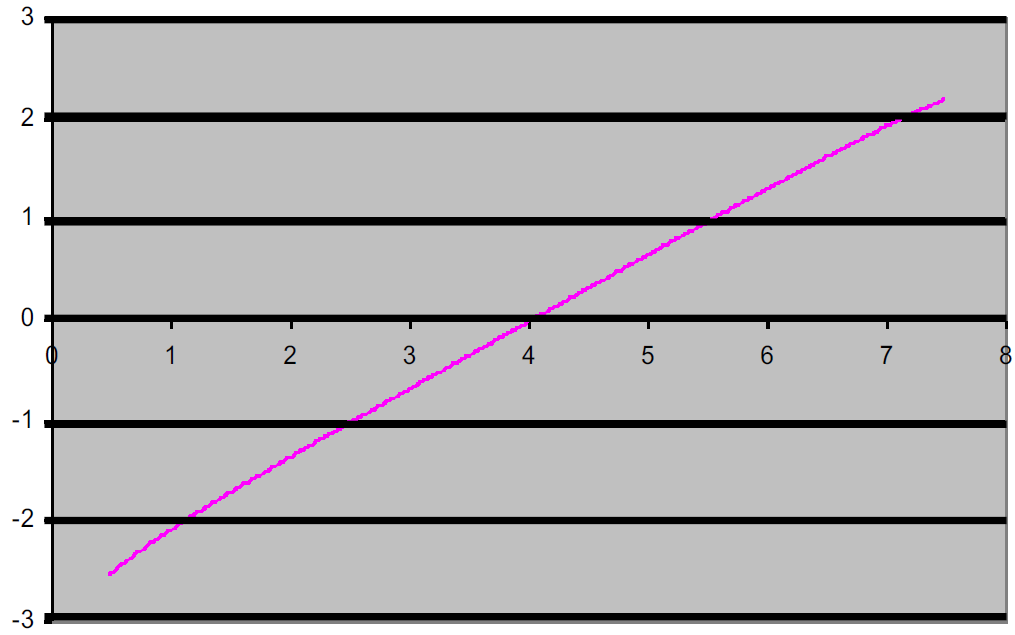
\includegraphics[width=0.45\textwidth,height=\textheight]{figuras/Papel5.png}
&
\(P\left[ \mu -\sigma <X<\mu +\sigma \right] = 0.683 \newline P\left[ \mu -2\sigma <X<\mu +2\sigma \right] = 0.954 \newline P\left[ \mu -3\sigma <X<\mu +3\sigma \right] = 0.997\) \\
\bottomrule()
\end{longtable}
\end{frame}

\begin{frame}{}
\protect\hypertarget{section-45}{}
\begin{block}{Ejercicio de Papel de probabilidad Normal}
\protect\hypertarget{ejercicio-de-papel-de-probabilidad-normal}{}
Se prueba la duración de un componente electrónico bajo condiciones de
temperatura alta para acelerar el mecanismo de falla. A continuación se
proporciona el tiempo de falla (en horas) de \(20\) componentes
seleccionados al azar. Haga una gráfica de los datos sobre papel de
probabilidad normal. ¿El tiempo de falla parece tener una distribución
normal?

\begin{table}
\centering\begingroup\fontsize{9}{11}\selectfont

\begin{tabular}{c|c|c|c}
\hline
176.1 & 24.7 & 34.9 & 133.8\\
\hline
76.6 & 55.0 & 122.8 & 99.6\\
\hline
150.4 & 73.0 & 90.6 & 131.5\\
\hline
197.6 & 124.5 & 2.4 & 40.4\\
\hline
35.3 & 155.7 & 46.0 & 40.4\\
\hline
\end{tabular}
\endgroup{}
\end{table}
\end{block}
\end{frame}

\begin{frame}{}
\protect\hypertarget{section-46}{}
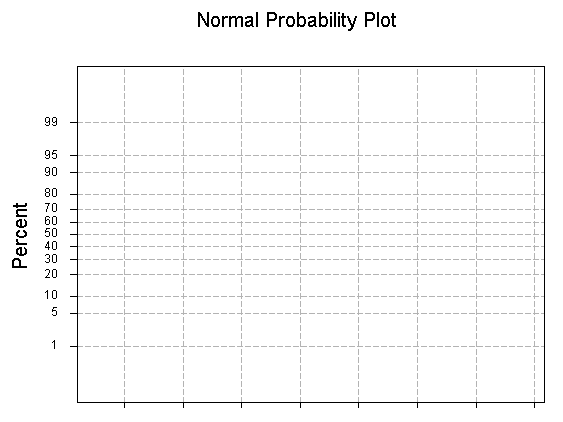
\includegraphics[width=2\textwidth,height=\textheight]{figuras/probpaperLandscape2.png}
\end{frame}

\begin{frame}{}
\protect\hypertarget{section-47}{}
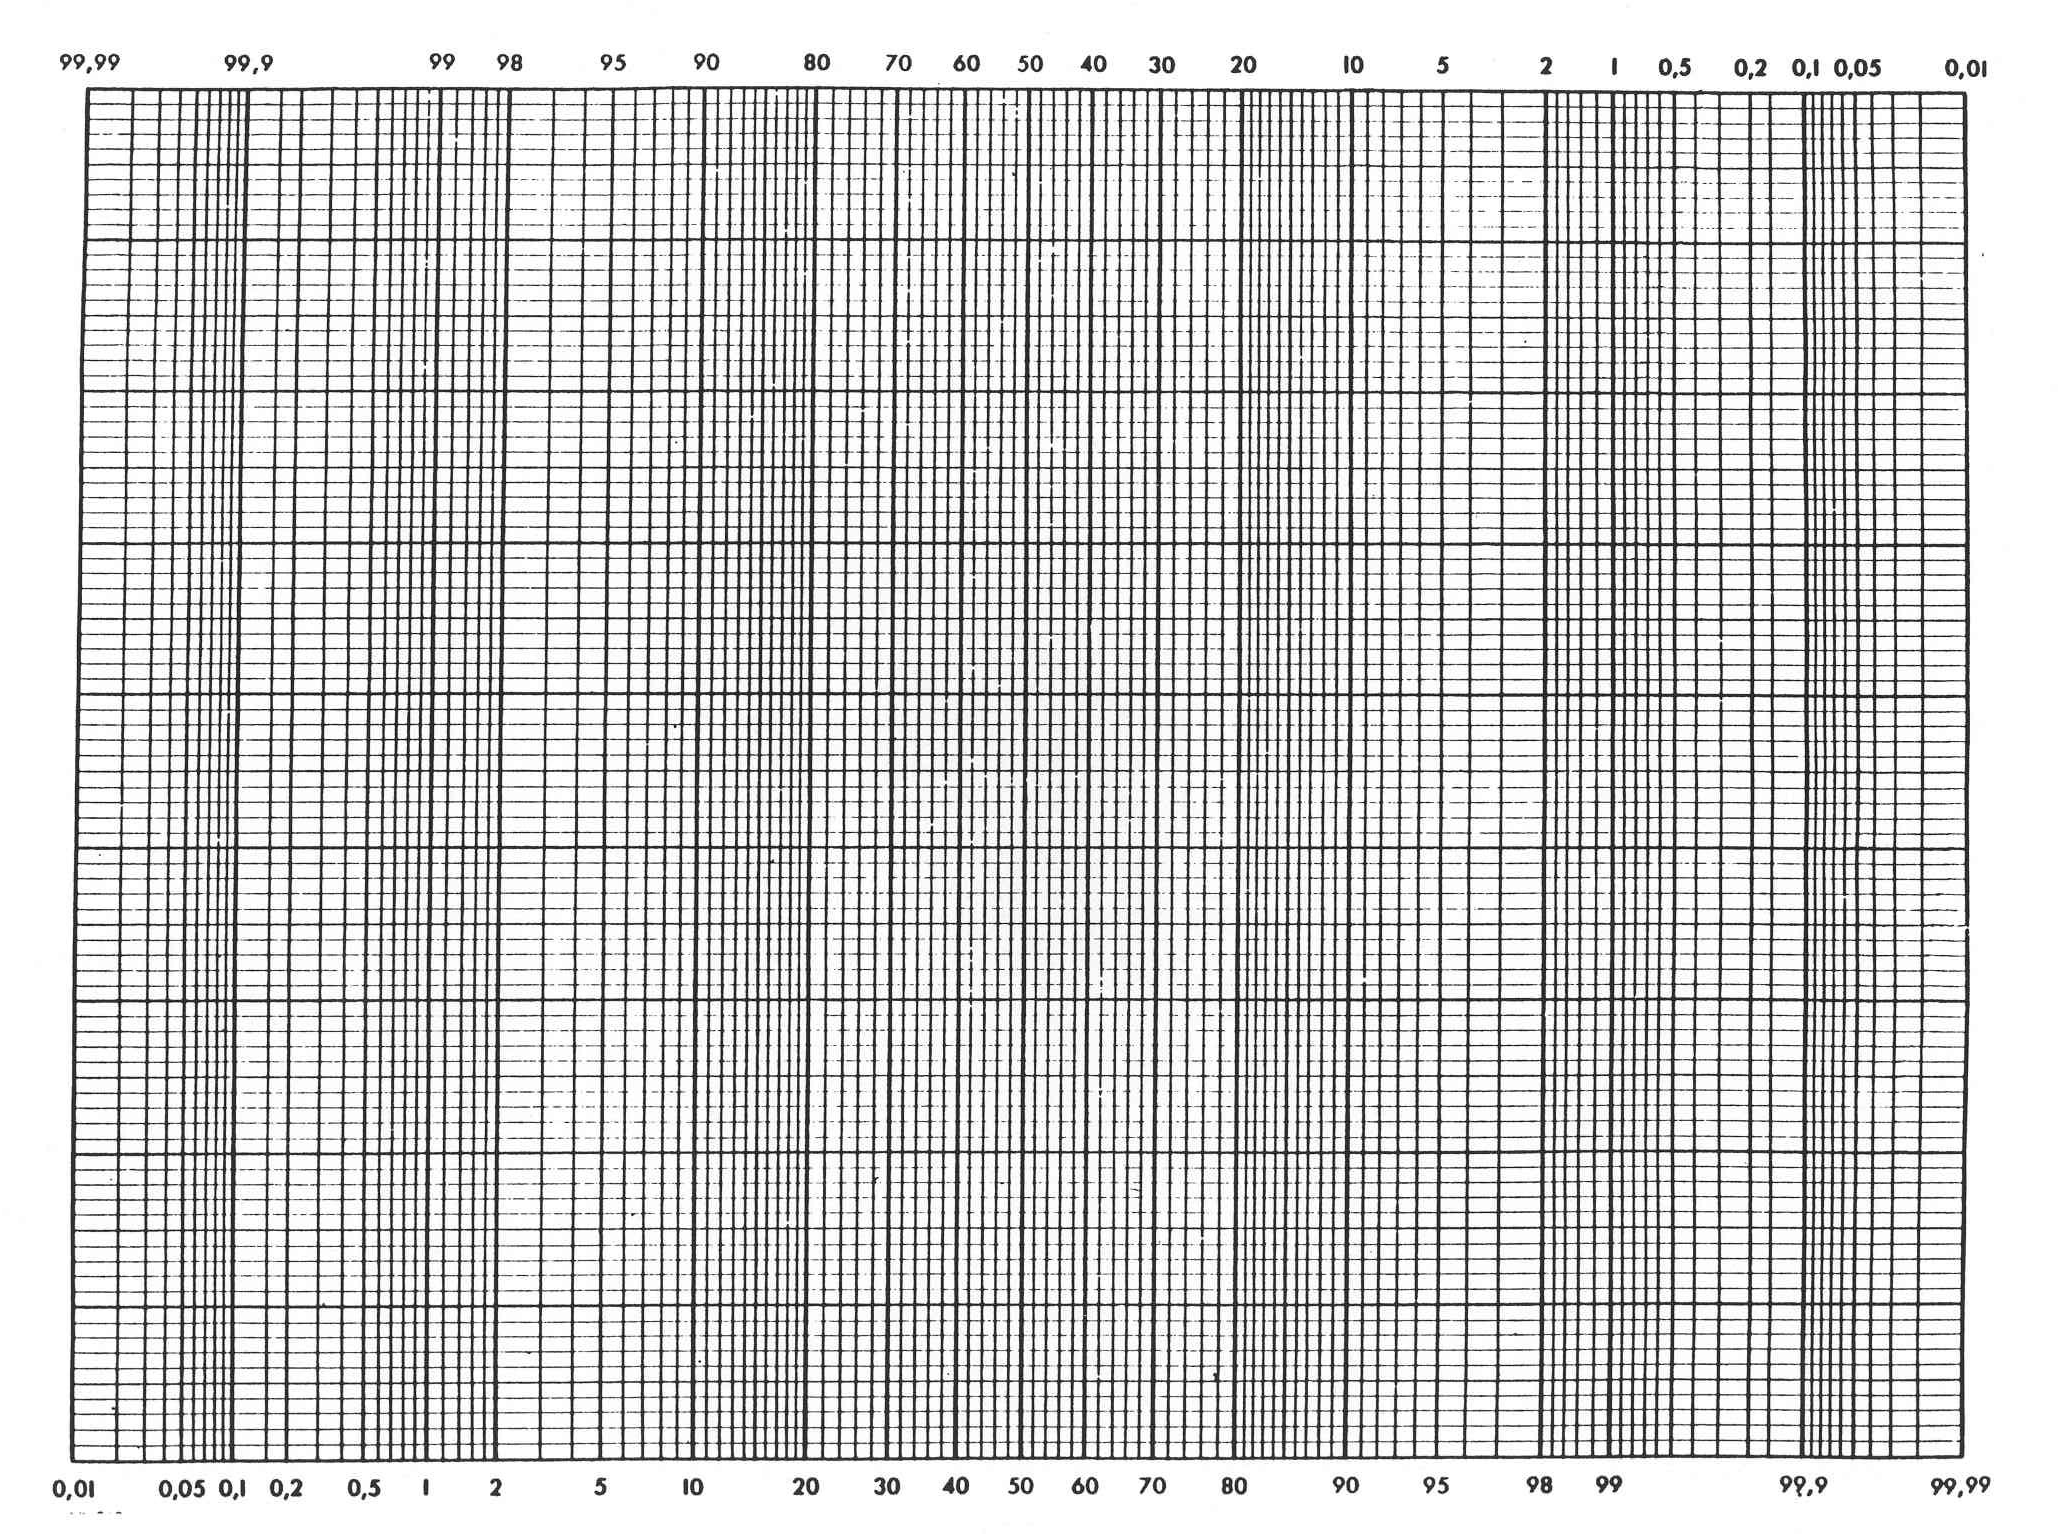
\includegraphics{figuras/probpaperLandscape.png}
\end{frame}

\begin{frame}{Gráfica de Probabilidad normal en R}
\protect\hypertarget{gruxe1fica-de-probabilidad-normal-en-r}{}
\begin{block}{Práctica}
\protect\hypertarget{pruxe1ctica}{}
\begin{itemize}
\item
  Realice la gráfica de probabilidad normal del ejemplo anterior.
\item
  Simule con \emph{semilla fija} datos con distribución Normal,
  Exponencial, Uniforme, t, Ji Cuadrada. Esto realícelo para tamaños de
  muestra de 15, 30, 50 y 100.
\item
  ¿Qué conclusiones puede obtener a partir de esta práctica?
\end{itemize}
\end{block}
\end{frame}

\begin{frame}{}
\protect\hypertarget{section-48}{}
Ver la siguiente aplicación en Shiny
\href{https://s3rgionava.shinyapps.io/QQnorm/?_ga=2.74771473.2040383487.1666298329-1276638344.1663958366}{qqnorm}

\begin{figure}
\centering
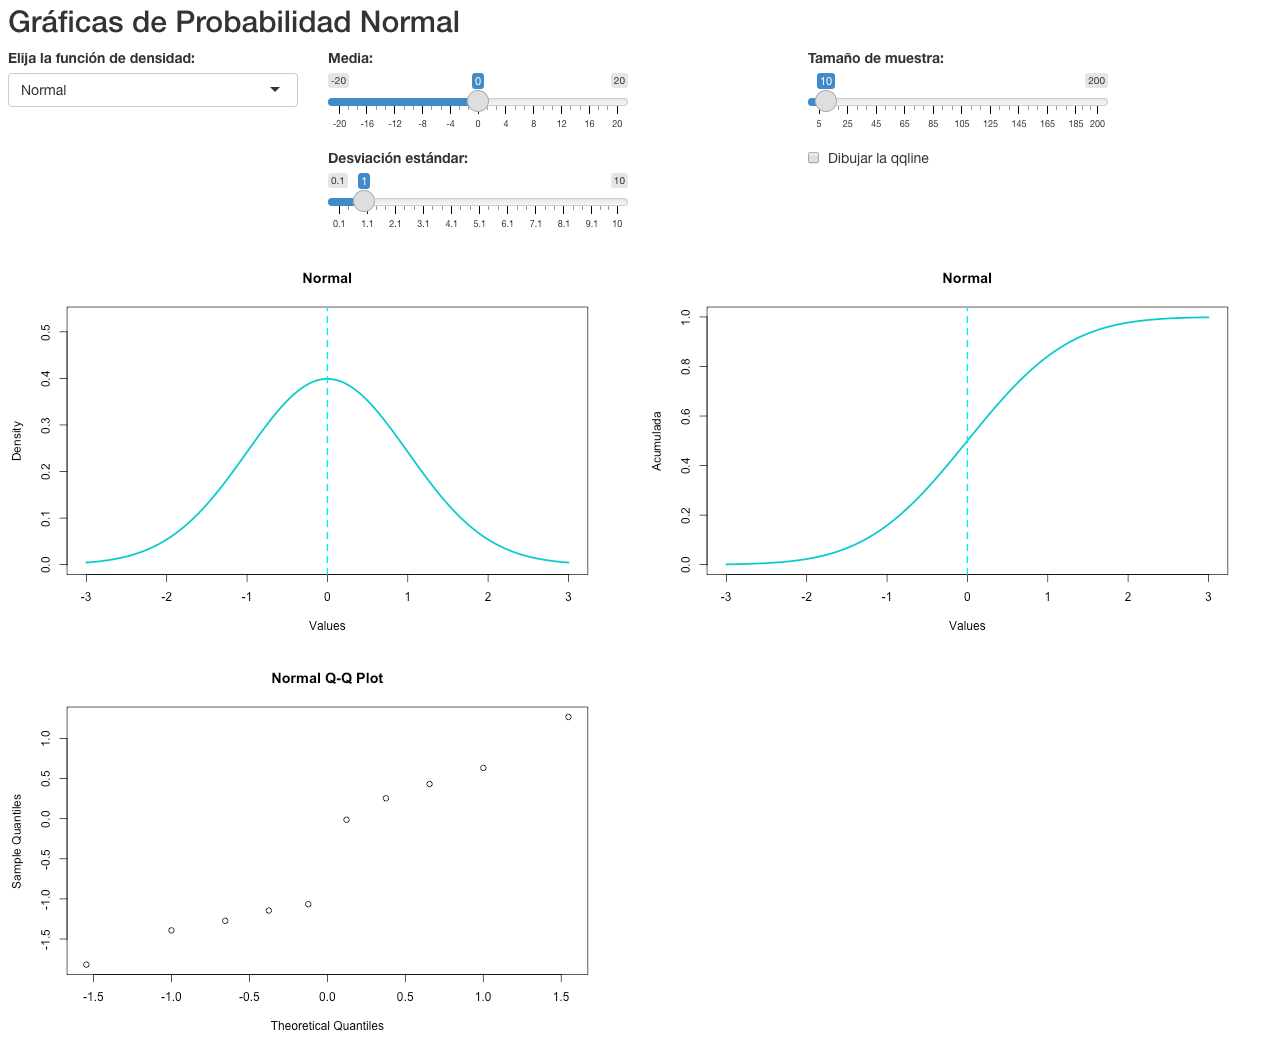
\includegraphics[width=0.7\textwidth,height=\textheight]{figuras/QQnorm.png}
\caption{Pantalla de Shiny app QQnorm}
\end{figure}
\end{frame}

\begin{frame}{}
\protect\hypertarget{section-49}{}
\begin{block}{¿Cómo se ven otras distribuciones muestrales?}
\protect\hypertarget{cuxf3mo-se-ven-otras-distribuciones-muestrales}{}
\begin{itemize}
\item
  Ejecute el archivo \textbf{distr\_muestral\_pequena2.R} en
  \url{https://rstudio.cloud/content/4731243} y discuta las salidas.
\item
  Simule la distribución muestral de la suma, mínimo y varianza para una
  población dada. La extracción será con reemplazo y con tamaño de
  muestra \(n\) fijo. Grafique la distribución muestral.
\item
  ¿Qué conclusiones puede obtener a partir de esta práctica?
\end{itemize}
\end{block}
\end{frame}

\begin{frame}{Distribución Ji-cuadrada (Chi-Square)}
\protect\hypertarget{distribuciuxf3n-ji-cuadrada-chi-square}{}
Hemos visto que el conocer la varianza \(\sigma^2\) resulta fundamental
para procedimientos de distribución muestral de la media, así como para
procedimientos de inferencia estadística.

Existen muchas aplicaciones prácticas en donde \(\sigma^2\) es el
objetivo primario de la investigación experimental. (Precisión en el
llenado de bolsas). En estos casos \(\sigma^2\) adquiere una mayor
importancia que la media de la población.

Las partes producidas por un proceso de manufactura deben ser producidas
con un mínimo de variabilidad para reducir el número de productos fuera
del rango aceptable (defectuosos). En general se desea mantener una
varianza mínima en las características de calidad de un producto
industrial para alcanzar el control del proceso y minimizar el
porcentaje de productos de baja calidad.
\end{frame}

\begin{frame}{}
\protect\hypertarget{section-50}{}
La varianza muestral

\[s^2=\frac{\sum_{i=1}^n (x_i -\bar{x})}{n-1}.\]

Es un estimador insesgado de la varianza de la población \(\sigma^2\).
La distribución muestral de \(s^2\), generada mediante muestras
repetidas, es una distribución de probabilidad que empieza en
\(s^2 = 0\) (ya que no puede ser negativa) con media igual a
\(\sigma^2\). La distribución \textbf{no es simétrica}.

La forma de la distribución depende del número de datos, así como de la
forma de la distribución de origen.
\end{frame}

\begin{frame}{}
\protect\hypertarget{section-51}{}
\begin{block}{En el caso de población normal}
\protect\hypertarget{en-el-caso-de-poblaciuxf3n-normal}{}
Si la población de origen de las muestras es normal, entonces la
distribución estandarizada que se obtiene es la Ji- cuadrada, calculada
como en la siguiente expresión:

\[\chi^2=\frac{(n-1)s^2}{\sigma^2}\]
\end{block}

\begin{block}{Relación de la Ji-cuadrada con la distribución normal}
\protect\hypertarget{relaciuxf3n-de-la-ji-cuadrada-con-la-distribuciuxf3n-normal}{}
Si \(Z \sim N(0,1)\), entonces \(Z^2\) tiene la distribución gama
especial a la que nos referimos como la distribución \(ji-cuadrada\) con
\(\nu = 1\) \textbf{grado de libertad}. La Ji-cuadrada es importante en
problemas de muestreo de poblaciones normales.

En general si \(Z_i \sim N(0,1)\), \(i=1,2,\ldots,n\) independientes,
entonces \[X=Z_1^2 +Z_2^2+\cdots+Z_n^2\] entonces \(X\sim\chi_n^2\).
\end{block}
\end{frame}

\begin{frame}{}
\protect\hypertarget{section-52}{}
\begin{block}{Distribución Ji-cuadrada}
\protect\hypertarget{distribuciuxf3n-ji-cuadrada}{}
Una variable aleatoria \(x\) tiene una distribución ji-cuadrada
(\(\chi^2\)) con \(\nu\) (nu) grados de libertad, si su densidad está
dada por:

\[f(x)=\frac{1}{2^{\frac{\nu}{2}}\Gamma(\nu/2)}x^{\frac{\nu-2}{2}}e^{-x/2} \mbox{ para } x>0\]
\end{block}

\begin{block}{Función Gama}
\protect\hypertarget{funciuxf3n-gama}{}
\[\Gamma(\alpha)=\int_0^\infty y^{\alpha -1}e^{-y}dy \qquad \mbox{ para } \alpha >0\]

Casos importantes: \(\Gamma(1/2)=\sqrt{\pi}\)

\(\Gamma(k)= (k-1)!\) para \(k\) entero.
\end{block}
\end{frame}

\begin{frame}{}
\protect\hypertarget{section-53}{}
\begin{center}\includegraphics{Distr-muestrales_files/figure-beamer/unnamed-chunk-19-1} \end{center}
\end{frame}

\begin{frame}{}
\protect\hypertarget{section-54}{}
\begin{block}{Estimación de Varianzas}
\protect\hypertarget{estimaciuxf3n-de-varianzas}{}
\textbf{Teorema}. Si \(s^2\) es la varianza de una muestra aleatoria de
tamaño \(n\) tomada de una población normal cuya varianza es
\(\sigma^2\), entonces:

\[\chi^2=\frac{(n-1)s^2}{\sigma^2}\] es el valor de una variable
aleatoria que tiene distribución Ji-cuadrada con parámetro
\(\gamma = \nu - 1\) grados de libertad.

\bigskip

Exactamente 95\% de una distribución chi cuadrada cae entre
\(\chi_{0.975}^2\) y \(\chi_{0.025}^2\). Un valor \(\chi^2\) que cae a
la derecha de \(\chi_{0.975}^2\) no tiene probabilidades de ocurrir, a
menos que el valor de \(\sigma^2\) que supusimos sea demasiado pequeño.
Lo mismo sucede con un valor \(\chi^2\) que cae a la izquierda de
\(\chi_{0.025}^2\), el cual tampoco es probable que ocurra, a menos que
el valor de \(\sigma^2\) que supusimos sea demasiado grande. En otras
palabras, es posible tener un valor \(\chi^2\) a la izquierda de
\(\chi_{0.025}^2\) o a la derecha de \(\chi_{0.975}^2\) cuando el valor
de \(\sigma^2\) es correcto; pero si esto sucediera, lo más probable es
que el valor de \(\sigma^2\) que se supuso sea un error.
\end{block}
\end{frame}

\begin{frame}{}
\protect\hypertarget{section-55}{}
\begin{block}{Ejemplo}
\protect\hypertarget{ejemplo-2}{}
Un fabricante de baterías para automóvil garantiza que su producto
durará, en promedio, \(3\) años con una desviación estándar de \(1\)
año. Si cinco de estas baterías tienen duraciones de
\(1.9, 2.4, 3.0, 3.5\mbox{ y }4.2\) años, ¿el fabricante continuará
convencido de que sus baterías tienen una desviación estándar de \(1\)
año? Suponga que las duraciones de las baterías siguen una distribución
normal.

\textbf{Solución}

Primero calculemos la media y varianza, muestrales:
\[\bar{x}=3 \qquad \mbox{y} \qquad s^2 = \frac{(1.9-3)^2 + (2.4-3)^2 + \cdots + (4.2-3)^2}{4}=0.815\]
Entonces \[\chi^2=\frac{(4)(0.815)}{1}=3.26\] es un valor de una
distribución chi cuadrada con \(4\) grados de libertad. Como \(95\%\) de
los valores \(\chi^2\) con \(4\) grados de libertad caen entre 0.484 y
11.143, el valor calculado con \(\sigma^2 = 1\) es razonable y, por lo
tanto, el fabricante no tiene razones para sospechar que la desviación
estándar no sea igual a \(1\) año.
\end{block}
\end{frame}

\begin{frame}{Distribución F}
\protect\hypertarget{distribuciuxf3n-f}{}
\begin{block}{Fisher-Snedecor}
\protect\hypertarget{fisher-snedecor}{}
Sí \(X_1 \sim \chi_{n_1}^2\) y \(X_2 \sim \chi_{n_2}^2\) y son
independientes y definimos \[X=\frac{X_1/n_1}{X_2/n_2}\] entonces
\(X \sim F_{n_1,n_2}\) a veces denotada como \(F(n_{1},n_{2})\) y su
función de densidad está dada por \[
f(x) = \frac{\Gamma((n_{1}+n_{2})/2)(n_{1}/n_{2})^{n_{1}/2}x^{n_{1}/2-1}}
{\Gamma(n_{1}/2)\Gamma(n_{2}/2)[(n_{1}/n_{2})x+1]^{(n_{1}+n_{2})/2}} \qquad \qquad x > 0,
\] para \(n_{1} = 1,2,\ldots\) y \(n_{2} = 1,2,\ldots \,\). La
distribución \(F\) se usa para inferencia estadística de razones de
varianzas de dos poblaciones normales. También se usa para inferencia
estadística de razones de tasas de dos poblaciones exponenciales.
\end{block}
\end{frame}

\begin{frame}{}
\protect\hypertarget{section-56}{}
\begin{center}\includegraphics{Distr-muestrales_files/figure-beamer/distF-1} \end{center}
\end{frame}

\end{document}
